\documentclass[a4paper,fleqn]{cas-sc}

\usepackage[utf8]{inputenc}
\usepackage[brazil]{babel}
\usepackage[authoryear,longnamesfirst]{natbib}
\usepackage{xcolor}
\usepackage{seqsplit}

% Permite que tags longas do Ollama quebrem dentro da célula da tabela.
\newcommand{\ollamatag}[1]{\texttt{\seqsplit{#1}}}

% Realce por coluna nas tabelas de resultados: melhor valor em verde, pior em vermelho.
\newcommand{\melhor}[1]{\textcolor{green!55!black}{#1}}
\newcommand{\pior}[1]{\textcolor{red!80!black}{#1}}

\renewcommand{\abstractname}{Resumo}

\begin{document}
\let\WriteBookmarks\relax
\def\floatpagepagefraction{1}
\def\textpagefraction{.001}

\shorttitle{LLMs para a Conversão de Normas da AEC para RASE}
\shortauthors{E. N. S. Brito et al.}

\title[mode=title]{Análise Comparativa de LLMs Open-Source para a Conversão de Normas de Arquitetura, Engenharia e Construção para o Formato RASE}

\author[1]{Eike Natan Sousa Brito}
\cormark[1]
\ead{eike.sousa@hotmail.com}
\credit{Conceituação, Metodologia, Software, Redação - rascunho original}

\author[1]{André Carvalho}
\ead{andre@dcomp.ufs.br}
\credit{Supervisão, Redação - revisão e edição}

\author[1]{Marco Antônio Brasiel Sampaio}
\ead{marco.sampaio@ufs.br}
\credit{Supervisão, Redação - revisão e edição}

\affiliation[1]{organization={Universidade Federal de Sergipe},
            addressline={Cidade Universitária Prof. José Aloísio de Campos},
            city={São Cristóvão},
            postcode={49100-000},
            state={Sergipe},
            country={Brasil}}

\cortext[1]{Autor correspondente}

\begin{abstract}
A metodologia \textit{Building Information Modeling} (BIM) organiza o planejamento e a execução de obras em torno de um modelo tridimensional detalhado, reduzindo retrabalho e antecipando interferências antes do início da construção. Esse modelo, porém, não resolve sozinho a verificação da conformidade dos projetos com as normas técnicas regulatórias, cuja natureza interpretativa torna a automação um problema em aberto. A metodologia RASE (\textit{Requirement, Applicability, Selection, Exception}) endereça essa lacuna ao reescrever cada trecho normativo como dado computável, permitindo que \textit{softwares} BIM verifiquem a conformidade automaticamente; a conversão das normas para esse formato, contudo, ainda é feita manualmente, regra a regra, o que se torna um gargalo para a automação. O Processamento de Linguagem Natural, em particular os Modelos de Linguagem de Grande Porte (LLMs), surge como caminho promissor para automatizar essa conversão, podendo ser adaptado à tarefa por meio da Engenharia de Prompt, técnica leve que ajusta apenas a instrução enviada ao modelo. Este trabalho avalia comparativamente seis LLMs \textit{open-source} (Llama, Dolphin, Gemma, Mistral, Alpaca e Qwen) na conversão automática de normas técnicas brasileiras da AEC para o formato RASE, utilizando exclusivamente Engenharia de Prompt em três níveis sucessivos de normalização (N1: segmentação atômica das sentenças normativas; N2: identificação dos operadores RASE; N3: estruturação semântica em JSON). A comparação foi conduzida em cinco experimentos (EN1, EN2, EN1N2, EN3 e EN1N2N3) sobre um \textit{dataset} de 79 normas anotadas da NBR~9050, com treze métricas distribuídas em cinco famílias (lexicais, semânticas, de distância, voltadas para geração e de classificação) e os modelos servidos localmente via Ollama, sob protocolo idêntico de \textit{dataset}, \textit{prompts} e \textit{hardware}. Os resultados mostram que a decomposição em três níveis, apoiada apenas em Engenharia de Prompt, é suficiente para gerar representações RASE válidas, alcançando similaridade semântica próxima de 0{,}90 nos melhores cenários; o Llama obteve a melhor média global (0{,}730), liderando as etapas do nível N3 (EN3 e EN1N2N3), enquanto o Dolphin apresentou a melhor relação custo-benefício, cerca de noventa vezes mais rápido no \textit{pipeline} encadeado.
\end{abstract}

\begin{keywords}[Palavras-chave]
Aprendizado de Máquina \sep Processamento de Linguagem Natural \sep LLM \sep Engenharia de Prompt \sep BIM \sep RASE
\end{keywords}

\maketitle

%% ======================================================================
\section{Introdução}\label{sec:introducao}
Projetar e revisar projetos de engenharia civil é uma atividade intensiva em conhecimento (\textit{knowledge-intensive activity}): exige que engenheiros interpretem normas, conciliem informações heterogêneas e tomem decisões fundamentadas em \textit{expertise} acumulada ao longo de anos de prática. A \textit{Engineering Informatics} estuda justamente como métodos computacionais podem apoiar essas atividades, transformando o conhecimento contido em documentos, modelos e normas em uma forma processável por máquina. Dentro desse campo, automatizar a verificação de projetos de edificações contra normas técnicas regulatórias é um problema antigo e ainda em aberto, já que essas normas são escritas em linguagem natural e exigem interpretação. O presente trabalho pode ser caracterizado como um problema dessa área: usa Inteligência Artificial (IA) para converter normas técnicas em uma representação computável que ferramentas \textit{Building Information Modeling} (BIM) possam verificar automaticamente, tarefa que se situa na interseção entre representação de conhecimento, Processamento de Linguagem Natural e a prática de engenharia.

Na engenharia civil brasileira, projetar e fiscalizar obras ainda envolve uma enorme quantidade de retrabalho. Parte desse desperdício vem da forma como os projetos são representados: o desenho 2D, padrão histórico do setor, esconde colisões e omite informações que só aparecem no canteiro. A migração para modelos tridimensionais e, mais especificamente, para a metodologia \textit{Building Information Modeling} (BIM) surgiu como resposta a esse problema \citep{eastman2011}.

O BIM organiza o planejamento e a execução da obra em torno de um modelo 3D detalhado. A metodologia divide-se em dimensões que vão do 3D ao 7D: 3D para o modelo geométrico; 4D para a programação temporal; 5D para custos; 6D para sustentabilidade; e 7D para a gestão da operação pós-construção \citep{eastman2011}. BIM não é um \textit{software}, e sim um conceito apoiado em sistemas informatizados como o CAD, implementado por ferramentas como o Revit (Autodesk) e o ArchiCAD (Graphisoft).

Modelar em BIM permite visualizar interferências antes do início da obra, reduzindo o retrabalho em campo. As aplicações típicas vão da análise de projetos ao orçamento, passando pelo planejamento, pela coordenação modular e pela gestão do ciclo de vida \citep{eastman2011}.

O BIM, porém, não resolve sozinho a verificação dos projetos contra as normas regulatórias. As normas regulatórias (ou técnicas) são documentos que estabelecem requisitos, critérios e procedimentos obrigatórios para assegurar a segurança, a qualidade e o desempenho das edificações; no Brasil, são editadas pela Associação Brasileira de Normas Técnicas (ABNT) na forma das NBRs, como a NBR~9050, voltada à acessibilidade. Cada jurisdição mantém seu próprio conjunto de regras, em geral redigidas em linguagem natural e de caráter interpretativo, o que torna a verificação automática de conformidade um problema em aberto \citep{dimyadi2013,solihin2015}.

Tornar essas normas verificáveis por máquina exige convertê-las em uma representação computável. Com essa finalidade, \citet{hjelseth2011} propuseram a metodologia RASE, que reescreve cada trecho normativo como dado estruturado, decomposto em quatro atributos: \textbf{R}equisito (o que precisa ser atendido), \textbf{A}plicabilidade (onde a regra se aplica), \textbf{S}eleção (opções para cumpri-la) e \textbf{E}xceção (casos em que a regra não vale). Uma vez organizada em RASE, a norma viabiliza ferramentas integradas a \textit{softwares} BIM, como o Revit, capazes de validar o projeto elemento a elemento \citep{santos2021}. O gargalo está antes disso: a conversão da norma para RASE ainda é feita manualmente, regra a regra, e, como um modelo BIM pode reunir centenas ou milhares de elementos sujeitos a normas, o custo desse trabalho cresce rapidamente.

Automatizar essa conversão exige reconhecer padrões em textos em linguagem natural, tarefa para a qual o Aprendizado de Máquina (AM) se mostra promissor. A motivação é reforçada pelo próprio BIM: quanto maior a adoção, maior o volume de dados gerado por cada projeto, o que atrai cientistas de dados, profissionais cuja função é transformar grandes volumes de informação em valor para as organizações \citep{davenport2012}. O AM, subárea da IA, estuda como construir algoritmos capazes de aprender padrões diretamente dos dados, sem programação explícita das regras \citep{tan2006}; a partir desses padrões, os modelos fazem previsões e respondem a situações novas. Na engenharia civil, a IA já automatiza etapas que antes dependiam de inspeção humana, da detecção de patologias em estruturas à previsão de prazos de obra \citep{rane2023,liu2022}.

Três exemplos recentes ilustram esse movimento. \citet{liu2022} combinaram BIM, AM e regras de \textit{design} para otimizar o processo de montagem da construção, com ganhos em eficiência e custo. \citet{alawadhi2023} treinaram Redes Neurais Artificiais sobre dados BIM para reconhecer objetos de construção em fotos: imagens sintéticas geradas a partir do modelo produziram segmentação semântica eficaz em fotografias reais, abrindo caminho para o uso de dados sintéticos em problemas arquitetônicos. Em outra frente, \citet{saka2024} alimentaram um modelo com 2.280 projetos de demolição para prever a circularidade de resíduos: o sistema estima as quantidades de material reciclável e destina os resíduos ao aterro adequado, apoiando o planejamento.

Quando o objeto de análise é o próprio texto normativo, a automação recai sobre o Processamento de Linguagem Natural (PLN), subárea da IA dedicada ao tratamento computacional da linguagem humana em tarefas como tradução, sumarização e classificação de texto. Dentro do PLN, a IA Generativa reúne os modelos capazes de produzir novos conteúdos (texto, imagem ou áudio) a partir do que aprenderam no treinamento. Entre suas manifestações mais relevantes estão os Modelos de Linguagem de Grande Porte (LLMs) \citep{zhao2023}, categoria que inclui o ChatGPT, da OpenAI \citep{openai2024}, e o Llama~3, da Meta \citep{llama3}.

Os LLMs são sistemas de IA voltados a entender e produzir linguagem humana em escala. O treinamento envolve volumes massivos de texto, o que permite ao modelo capturar nuances linguísticas e contextuais. Quase todos os LLMs atuais usam alguma variação da arquitetura \textit{transformer}, escolhida por sua eficiência no processamento de sequências longas \citep{zhao2023}.

A adaptação desses modelos a domínios específicos pode seguir caminhos diferentes. O mais leve e acessível é a Engenharia de Prompt (EP): em vez de retreinar pesos ou montar uma infraestrutura de recuperação, ajusta-se apenas a instrução enviada ao modelo.

No setor AEC, os LLMs podem auxiliar tanto na leitura das normas quanto na sua conversão para formatos processáveis por máquina \citep{fuchs2024}. A literatura, porém, ainda tem lacunas: uma delas é justamente a interpretação de leis, códigos e padrões regulatórios, cuja complexidade semântica historicamente desafiou os métodos de IA anteriores \citep{fuchs2024}.

Diante dessa lacuna, este trabalho decompõe a conversão de normas para RASE em três níveis sucessivos de normalização, apoiados unicamente em Engenharia de Prompt: o nível \textbf{N1} segmenta a sentença normativa em regras atômicas; o \textbf{N2} identifica, em cada regra, os operadores RASE; e o \textbf{N3} estrutura o resultado em JSON. Sobre essa decomposição, comparam-se seis LLMs \textit{open-source} (Llama, Dolphin, Gemma, Mistral, Alpaca e Qwen), servidos localmente, em cinco experimentos que avaliam cada nível isoladamente e em \textit{pipeline} encadeado. A qualidade das saídas é aferida por nove métricas de similaridade textual em quatro famílias: lexicais (FuzzyWuzzy e TF-IDF), semânticas (SBERT, BERTimbau e Multilingual), de distância (\textit{Word Mover's Distance} com FastText e NILC) e voltadas para geração (BERTScore e ROUGE-L); a essas somam-se quatro métricas de classificação (Acurácia, Precisão, Revocação e F1-score).

As contribuições deste trabalho situam-se na interseção entre Arquitetura, Engenharia e Construção (AEC) e Computação: para a AEC, aplica modelos de PLN à checagem de normas de construção e propõe níveis sucessivos de normalização sobre a metodologia RASE de \citet{hjelseth2011}; para a Computação, leva LLMs consolidados na literatura a um novo domínio e os submete a uma avaliação sistemática de desempenho.

\section{Background}\label{sec:background}

\subsection{Normas de Engenharia e a Metodologia RASE}\label{sec:normas-rase}
As normas técnicas formam o arcabouço regulatório do setor AEC: definem os requisitos mínimos de segurança, desempenho, qualidade e interoperabilidade dos projetos. No plano internacional, a Organização Internacional de Padronização (ISO) publica normas adotadas por diversos países; em BIM, a referência consolidada é a série ISO~19650, voltada à organização e à digitalização da informação sobre obras de construção \citep{iso19650}. Independentemente da jurisdição, cada norma combina três camadas textuais: (i) definições e referências, sem valor de verificação direta; (ii) requisitos prescritivos, com limites numéricos e geométricos passíveis de checagem automática; e (iii) recomendações e exceções, em texto livre, frequentemente condicionadas a categorias específicas do edifício. Em qualquer das três camadas o texto bruto é longo, recursivo e fortemente dependente de definições prévias, o que torna a tradução para regras computáveis um trabalho não trivial e, hoje, predominantemente manual.

A aplicação dessas normas permanece, em grande parte, manual: o profissional lê trechos longos de texto, identifica os requisitos pertinentes e verifica item a item contra o projeto. Em um modelo BIM com centenas ou milhares de elementos sujeitos a normas simultâneas, esse esforço cresce de forma combinatória; \citet{eastman2009} mostram que a verificação manual é cara, frágil e pouco escalável, motivando a pesquisa em checagem automática baseada em regras. Automatizá-la, porém, esbarra em três obstáculos: a ambiguidade e as referências cruzadas da linguagem natural em que as normas são escritas \citep{dimyadi2013}; a variação regional, que limita o reaproveitamento do que já foi formalizado em outros contextos \citep{dimyadi2013,solihin2015}; e a dificuldade semântica de distinguir, dentro de um trecho, o que é requisito, aplicabilidade e exceção, o que exige um esquema padronizado e interoperável entre ferramentas \citep{solihin2015}.

A resposta que a literatura vem consolidando é estruturar a norma em um esquema computável antes da verificação. \citet{beach2015} demonstram que um sistema baseado em regras automatiza a checagem regulatória da construção quando as normas estão formalizadas. Nessa direção, \citet{hjelseth2015} propôs duas metodologias complementares: a Tx3 e a RASE. A Tx3 classifica cada informação do regulamento em \textbf{Transcrever} (instruções diretamente transcritíveis em regras computáveis), \textbf{Transformar} (instruções que precisam ser reescritas preservando o sentido) e \textbf{Transferir} (requisitos imprecisos, que exigem análise de um especialista). Os elementos transcritíveis e transformáveis são reescritos e submetidos à RASE, que marca cada trecho normativo em quatro operadores lógicos \citep{hjelseth2011}: \textbf{R}equisito (o dever associado, em geral expresso pelo imperativo ``deve''), \textbf{A}plicabilidade (a quem ou ao que o requisito se aplica), \textbf{S}eleção (um subconjunto da aplicabilidade) e \textbf{E}xceção (os casos excluídos da regra). Cada operador recebe ainda atributos estruturados, como objeto, propriedade, comparador, valor e unidade, o que aproxima o texto de uma forma diretamente verificável. Por exemplo, na sentença ``a inclinação transversal deve ser de até 2\% para pisos internos'', a aplicabilidade é ``pisos'', a seleção ``internos'' e o requisito ``inclinação transversal menor ou igual a 2\%''. Uma vez organizada em RASE, a norma viabiliza ferramentas integradas a \textit{softwares} BIM, como o Revit, capazes de validar o projeto elemento a elemento \citep{santos2021}. Aplicar a RASE manualmente, contudo, reintroduz o gargalo que se quer eliminar: marcar operador a operador exige um especialista e não escala para o volume de normas do setor. No fundo, identificar Requisito, Aplicabilidade, Seleção e Exceção em uma sentença é um problema de classificação e de estruturação de texto, exatamente o tipo de tarefa que técnicas de Aprendizado de Máquina aprendem a partir de exemplos.

\subsection{Modelos de Linguagem de Grande Porte e Métricas de Validação Textual}\label{sec:llm-metricas}
Modelos de Linguagem de Grande Porte (LLMs) são modelos de IA que combinam Aprendizado de Máquina, redes neurais profundas e técnicas de Processamento de Linguagem Natural para entender e gerar linguagem humana \citep{touvron2023}. São tipicamente pré-treinados de forma não supervisionada sobre bilhões de palavras, aprendendo a prever a estrutura das sentenças por probabilidade, e adotam a arquitetura \textit{Transformer} \citep{vaswani2017}, eficiente no tratamento de dependências contextuais em sequências longas. O lançamento do ChatGPT e do GPT-4 \citep{openai2024} popularizou esses modelos, e, como resposta a modelos fechados, surgiram alternativas de pesos abertos como o LLaMA \citep{touvron2023,llama3}. Entre as técnicas que especializam um LLM para uma tarefa de domínio sem alterar seus pesos, a Engenharia de Prompt é a mais leve: consiste em desenhar com cuidado a instrução enviada ao modelo, prática essencial para extrair respostas adequadas ao contexto \citep{brown2020}.

Avaliar a saída de um LLM em tarefas de conversão de texto exige compará-la a uma referência. Como a correspondência exata raramente é desejável, já que uma paráfrase correta também deve contar como acerto, emprega-se um conjunto de métricas de similaridade, organizadas em quatro famílias \citep{jurafsky2009}. As \textbf{lexicais} comparam a forma de superfície das \textit{strings}: a \textit{FuzzyWuzzy}, baseada na distância de Levenshtein, e a similaridade do cosseno sobre vetores TF-IDF \citep{manning2008}. As \textbf{semânticas} apoiam-se em \textit{sentence embeddings} que aproximam textos de sentido equivalente, como o \textit{Sentence-BERT} \citep{reimers2019}, o BERTimbau (especializado em português) \citep{souza2020} e modelos multilíngues. As \textbf{de distância} medem o custo de alinhar os \textit{embeddings} das palavras de um texto aos do outro, caso da \textit{Word Mover's Distance} \citep{kusner2015}, executável sobre \textit{embeddings} do FastText \citep{bojanowski2017} ou do projeto NILC. As \textbf{voltadas para geração}, originárias da tradução automática e da sumarização, medem o quanto a saída reproduz a referência: o \textit{BERTScore} \citep{zhang2020bertscore}, que alinha \textit{tokens} por similaridade contextual, e o \textit{ROUGE-L} \citep{lin2004rouge}, baseado na maior subsequência comum. A essas somam-se métricas de classificação (acurácia, precisão, revocação e \textit{F1-score}), derivadas da matriz de confusão, que tornam explícitas omissões e alucinações ao tratar a avaliação como um problema de extração de informação \citep{manning2008}.

\subsection{Trabalhos Relacionados}\label{sec:trabalhos-relacionados}
A integração do BIM com tecnologias de IA generativa ainda é pouco explorada no setor AEC, mas é objeto de uma onda recente de trabalhos. \citet{rane2023} analisam a integração entre BIM e modelos como ChatGPT e Bard, identificando ganhos em \textit{design} e tomada de decisão, mas apontando obstáculos persistentes (falta de padronização dos dados, deficiências de segurança e dificuldade dos modelos em interpretar a semântica de dados BIM) e propondo um \textit{framework} de adoção. \citet{lin2023} apresentam o JULE, um \textit{chatbot} que combina BIM e PLN para entregar, no canteiro, consultas em tempo real sobre dimensões de componentes sem abrir as interfaces convencionais, com alta precisão na identificação de intenção, mas condicionado a dados BIM bem estruturados. \citet{sammou2024} aplicam GPT-3.5 e GPT-4 a 385 questões de segurança e três técnicas de Engenharia de Prompt (\textit{Prompt Direct}, \textit{Chain-of-Thought} e \textit{Few-Shot}): o GPT-4 atingiu 84,6\% de acerto contra 73,8\% do GPT-3.5, mas ambos falharam em questões de emergência e cálculo, expondo a fragilidade da confiabilidade técnica. Por fim, \citet{samsami2024} mostram que \textit{prompts} genéricos não funcionam no setor AEC e que \textit{prompts} específicos reduzem erros, embora alucinações em tarefas complexas e a necessidade de validação externa persistam. No conjunto, os trabalhos confirmam o potencial dos LLMs no setor, mas revelam uma lacuna comum: a ausência de uma representação estruturada e formal que traduza o conteúdo normativo em regras computáveis. Sem ela, os LLMs extraem texto e geram \textit{insights}, mas não convertem a norma em algo diretamente verificável por máquina, exatamente o ponto que este trabalho procura endereçar ao acoplar os LLMs à metodologia RASE.

\section{RASE-PE: Conversão de Normas para RASE com Engenharia de Prompt}\label{sec:metodologia}
A metodologia proposta, aqui denominada \textbf{RASE-PE}, sustenta-se em três decisões: (i) decompor a conversão de normas para o formato RASE em três níveis sucessivos de normalização (N1, N2 e N3); (ii) usar a Engenharia de Prompt como única técnica de especialização dos modelos, sem alterar pesos nem infraestrutura de recuperação; e (iii) comparar sistematicamente seis LLMs \textit{open-source} servidos localmente via Ollama, sob protocolo idêntico de \textit{dataset}, \textit{prompts} e \textit{hardware}. As subseções a seguir detalham a decomposição em três níveis, a Engenharia de Prompt empregada, os modelos avaliados, o \textit{dataset}, as métricas de validação e, por fim, o ambiente computacional e a estrutura do código.

\subsection{Normalização em Três Níveis}\label{sec:tres-niveis}
Sair do texto bruto de uma norma e chegar à representação RASE em JSON exige três raciocínios distintos: segmentação sintática, classificação semântica e extração de atributos estruturados. Pedir tudo em uma única chamada ao LLM tende a degradar a saída, com alucinações, omissões e JSONs inválidos. O RASE-PE decompõe a tarefa em três níveis sucessivos, isolando cada decisão e permitindo validar cada etapa em separado:

\begin{itemize}
\item \textbf{N1: Segmentação Atômica.} Sentenças normativas costumam embutir mais de uma regra coordenada (por exemplo, ``a inclinação transversal deve ser de até 2\% para pisos internos e de até 3\% para pisos externos'' contém duas regras). O N1 quebra a sentença original em itens atômicos, com uma única regra por item, condição para que as etapas seguintes atribuam corretamente os operadores RASE.
\item \textbf{N2: Identificação dos Operadores RASE.} A partir de cada regra atômica, o N2 identifica quais trechos correspondem a Requisito, Aplicabilidade, Seleção e Exceção. É o núcleo da formalização: sem ele, o texto permanece em linguagem natural.
\item \textbf{N3: Estruturação Semântica em JSON.} Classificar um trecho como R, A, S ou E ainda o deixa em linguagem natural; para a verificação automática contra um modelo BIM é preciso extrair os dados para campos estruturados. O N3 produz um JSON com os campos \textit{type}, \textit{object}, \textit{property}, \textit{comparation}, \textit{target} e \textit{unit}.
\end{itemize}

O encadeamento N1~$\rightarrow$~N2~$\rightarrow$~N3 forma o \textit{pipeline} completo do RASE-PE (Figura~\ref{img:pipeline}), do texto bruto à representação RASE estruturada. Para isolar a contribuição de cada nível e medir a propagação de erros ao longo da cadeia, a avaliação é organizada em cinco experimentos, apresentados na Seção~\ref{sec:resultados}.

\begin{figure}[ht]
\centering
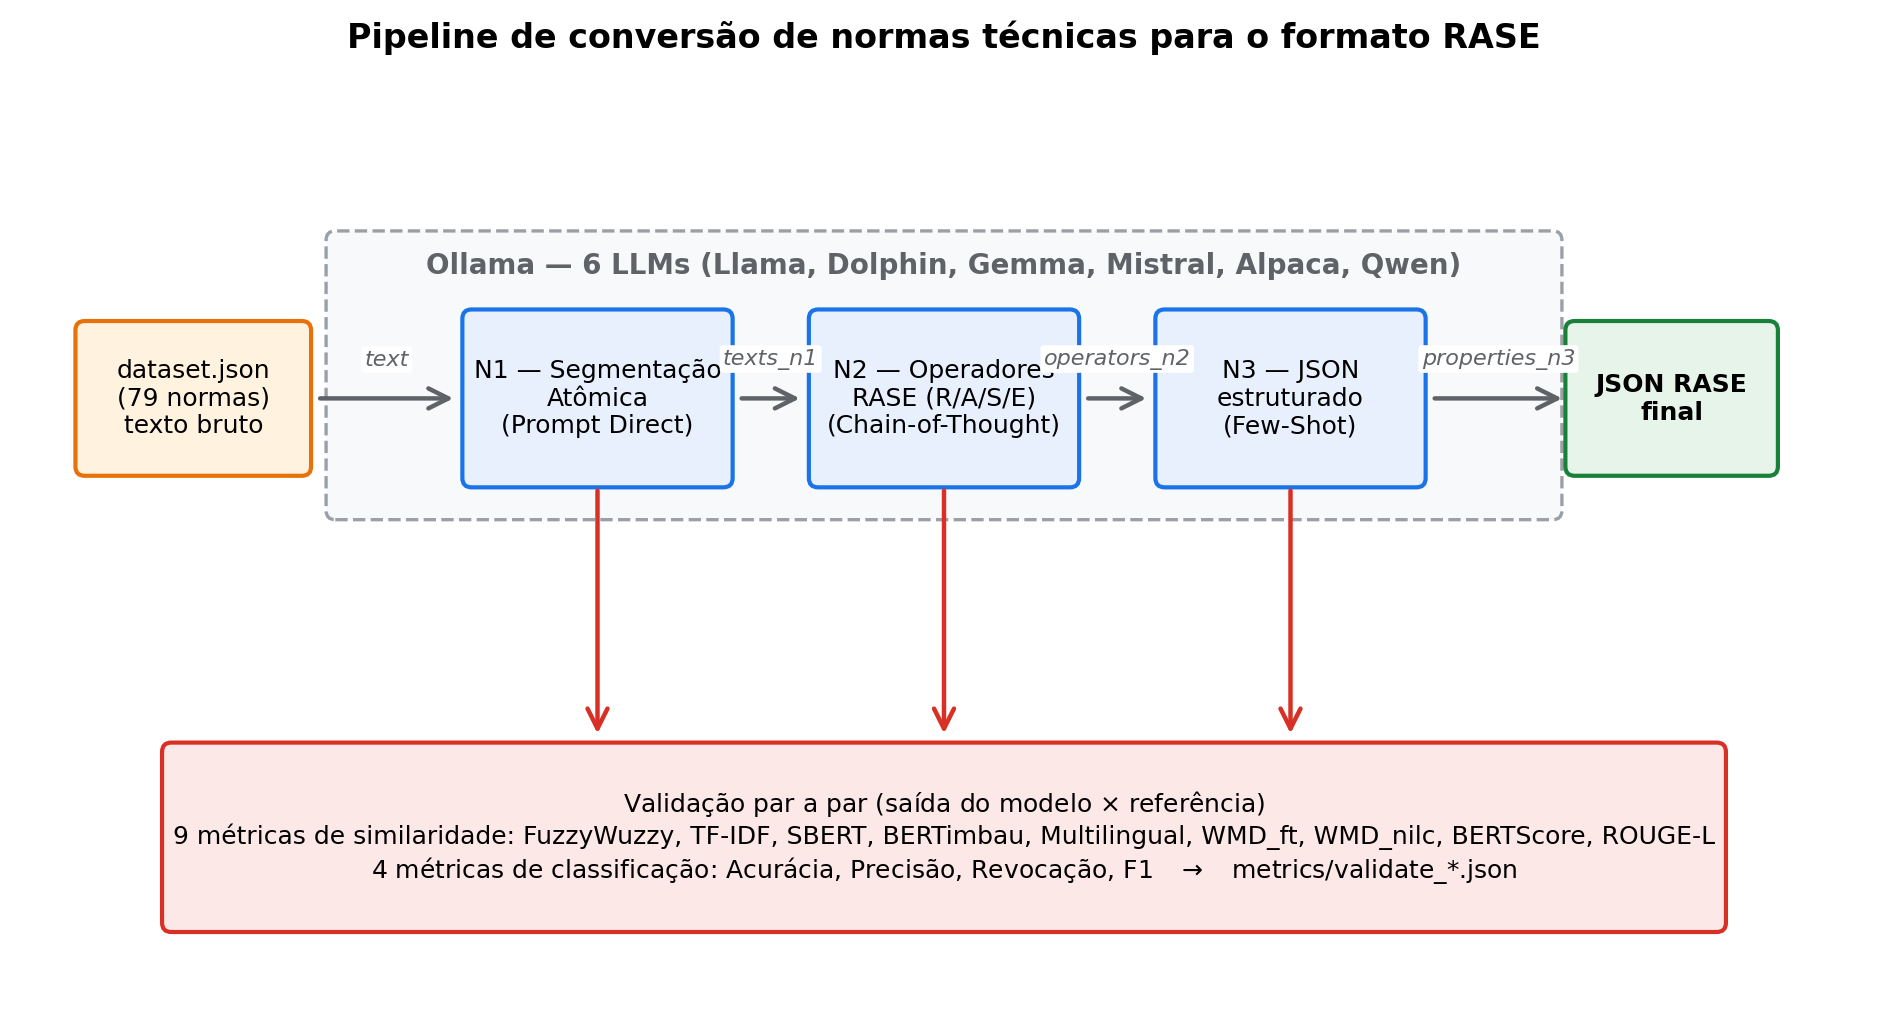
\includegraphics[width=0.98\linewidth]{figs/pipeline.png}
\caption{\textit{Pipeline} RASE-PE de conversão de normas técnicas para o formato RASE.}
\label{img:pipeline}
\end{figure}

\subsection{Engenharia de Prompt}\label{sec:engenharia-prompt}
A especialização dos LLMs foi feita exclusivamente por Engenharia de Prompt: toda a adaptação à tarefa vive nos \textit{prompts}, organizados por nível e por operador. Três técnicas clássicas foram aplicadas, cada uma escolhida pela natureza do nível em que atua. O \textbf{N1} usa \textit{Prompt Direct}, uma instrução direta e objetiva, adequada a uma tarefa estruturalmente simples (segmentar a sentença em sub-regras) e econômica em \textit{tokens} e latência. O \textbf{N2} usa \textit{Chain-of-Thought}, pedindo ao modelo que explicite o raciocínio em etapas antes de responder, o que reduz alucinações ao classificar trechos com múltiplos operadores. O \textbf{N3} usa \textit{Few-Shot}, embutindo exemplos completos de entrada e saída que ancoram o esquema JSON rígido; como cada operador RASE tem natureza distinta, adotou-se um \textit{prompt} por operador (Aplicabilidade, Requisito, Seleção e Exceção), cada um com o esquema de saída, heurísticas de mapeamento por padrões textuais comuns (por exemplo, ``uso público'' $\rightarrow$ \textit{property} ``uso'', \textit{comparation} ``='', \textit{target} ``público'') e exemplos próprios.

\subsection{Modelos LLM Avaliados}\label{sec:modelos}
Foram avaliados seis modelos \textit{open-source}, executados localmente via Ollama \citep{ollama2024}, escolhidos por representarem perfis complementares de peso, alinhamento, idioma e foco de \textit{fine-tuning} (Tabela~\ref{tab:modelos}). Todos compartilham a arquitetura \textit{Transformer} decodificadora e o paradigma de pré-treinamento massivo seguido de pós-treinamento por instruções, mas diferem em dados, alinhamento e escala. Salvo o Llama, avaliado em sua versão oficial multilíngue de propósito geral, todos foram executados a partir de \textit{checkpoints} adaptados ao português brasileiro publicados por terceiros e disponíveis no registro do Ollama. Executar os seis modelos no mesmo \textit{hardware}, com os mesmos \textit{prompts} e o mesmo \textit{dataset}, é o que garante a comparabilidade entre os resultados.

\begin{table}[ht]
\centering
\caption{Modelos LLM \textit{open-source} avaliados, com origem e \textit{tag} servida via Ollama.}
\label{tab:modelos}
\footnotesize
\setlength{\tabcolsep}{4pt}
\begin{tabular}{@{}l l >{\raggedright\arraybackslash}p{5.3cm} l@{}}
\toprule
Modelo & Origem & Tag servida via Ollama & Parâmetros \\
\midrule
Llama   & Meta                     & \ollamatag{llama3.1:8b}                                  & 8B \\
Dolphin & cnmoro (LLaMA-3 PT)      & \ollamatag{cnmoro/llama-3-8b-dolphin-portuguese-v0.3:4\_k\_m} & 8B (Q4\_K\_M) \\
Gemma   & brunoconterato (PT-BR)   & \ollamatag{brunoconterato/Gemma-3-Gaia-PT-BR-4b-it:f16}  & 4B (FP16) \\
Mistral & cnmoro (PT)              & \ollamatag{cnmoro/mistral\_7b\_portuguese:q4\_K\_M}      & 7B (Q4\_K\_M) \\
Alpaca  & splitpierre (Bode PT-BR) & \ollamatag{splitpierre/bode-alpaca-pt-br:13b-Q4\_0}      & 13B (Q4\_0) \\
Qwen    & cnmoro (PT)              & \ollamatag{cnmoro/Qwen2.5-0.5B-Portuguese-v1:q4\_k\_m}   & 0,5B (Q4\_K\_M) \\
\bottomrule
\end{tabular}
\end{table}

\subsection{\textit{Dataset}}\label{sec:dataset}
O \textit{dataset} foi consolidado em um único arquivo JSON com \textbf{79 normas anotadas}, oriundas de regulamentações brasileiras da AEC, com ênfase na NBR~9050 \citep{abnt9050}, adaptadas a partir do trabalho de \citet{eduardo2020}. A NBR~9050 foi escolhida por seu perfil majoritariamente prescritivo, com valores numéricos diretamente verificáveis em um modelo BIM e exceções bem delimitadas. Cada entrada reúne a decomposição RASE de referência nos três níveis: o texto bruto da norma (\texttt{text}); a lista de regras atômicas (\texttt{texts\_n1}); para cada regra, os quatro operadores RASE (\texttt{operators\_n2}, com as chaves \texttt{requeriments}, \texttt{aplicability}, \texttt{selection} e \texttt{exception}); e, para cada operador, o trecho classificado (\texttt{text\_n2}) e as propriedades estruturadas em JSON (\texttt{properties\_n3}). Operadores ausentes preservam a estrutura com \textit{strings} vazias. O mesmo arquivo serve de entrada para os geradores e de referência para os validadores, simplificando a reprodutibilidade.

\subsection{Métricas de Validação}\label{sec:metricas}
A avaliação combina treze métricas em cinco famílias. As nove métricas de \textbf{similaridade} (apresentadas na Seção~\ref{sec:llm-metricas}) são calculadas par a par entre a saída prevista e a referência, sempre na escala normalizada $[0,1]$: similaridade lexical (FuzzyWuzzy e TF-IDF), semântica (SBERT-PT \texttt{tgsc/sentence-transformer-ult5-pt-small}, Legal-BERTimbau e \texttt{paraphrase-multilingual-mpnet-base-v2}), de distância (WMD sobre \textit{embeddings} do FastText e do NILC) e voltadas para geração (BERTScore e ROUGE-L). A elas somam-se quatro métricas de \textbf{classificação} (acurácia, precisão, revocação e \textit{F1-score}), que tratam a avaliação como extração de informação e tornam explícitas omissões e alucinações. Um elemento é \textit{positivo} quando preenchido e \textit{negativo} quando vazio (\verb|""|); o critério de ``casamento'' é a similaridade semântica acima de um limiar de 0{,}7 em N1 e N2, e a igualdade exata (após normalização de caixa, acentos e pontuação) em N3. O limiar de 0{,}7 equilibra rigor e tolerância a paráfrases legítimas; como é aplicado igualmente a todos os modelos e experimentos, preserva a comparabilidade relativa entre eles.

\subsection{Ambiente Computacional e Implementação}\label{sec:ambiente}
Todas as execuções foram conduzidas em uma única estação de trabalho (CPU Intel Core i9-13900K, 32~GB de RAM, GPU NVIDIA RTX~4080, Ubuntu~22.04, Python~3.11), com os modelos servidos pelo Ollama (\texttt{ollama serve}) e as métricas calculadas com \texttt{sentence-transformers}, \texttt{gensim}, \texttt{fuzzywuzzy} e \texttt{scikit-learn}. O \textit{pipeline} foi implementado como um projeto Python modular, orquestrado por um \textit{script} principal que expõe três caminhos (geração de dados, validação e geração de tabelas). O código organiza-se em pacotes por responsabilidade: \texttt{config/} (registro dos modelos e conexão com o Ollama), \texttt{prompts/} (os \textit{prompts} em arquivos de texto, um por nível e um por operador no N3), \texttt{generates/} e \texttt{validates/} (um módulo por etapa, com estrutura simétrica), \texttt{utils/} (rotinas auxiliares de limpeza, emparelhamento e cálculo das métricas) e o \texttt{dataset.json} anotado. Essa separação mantém cada nível isolado e torna o \textit{pipeline} reprodutível: trocar de modelo significa apenas alterar uma entrada de configuração, e cada experimento pode ser regenerado ou revalidado de forma independente. O código-fonte completo está disponível em \url{https://github.com/EikESousA/Rase-PE}.

\section{Resultados e Discussão}\label{sec:resultados}

Esta seção apresenta os resultados da aplicação dos seis LLMs \textit{open-source} sobre as 79 normas brasileiras do \textit{dataset}, nos cinco experimentos: EN1 (segmentação N1 isolada), EN2 (identificação RASE com N1 de referência), EN1N2 (\textit{pipeline} encadeado N1$\rightarrow$N2), EN3 (estruturação JSON em isolamento, com N2 de referência) e EN1N2N3 (\textit{pipeline} encadeado completo N1$\rightarrow$N2$\rightarrow$N3). Todos os números vêm diretamente dos arquivos \textit{metrics/validate\_*.json}, gerados pela rotina de validação descrita na Seção~\ref{sec:metricas}. Para cada experimento, o texto traz as médias agregadas por métrica, os resultados detalhados por modelo, os tempos de execução e uma discussão integrada.

\textbf{Convenção de leitura das tabelas.} Em todas as tabelas numéricas desta seção, o realce é feito \textbf{por coluna}: o melhor valor de cada coluna aparece em \melhor{verde} e o pior em \pior{vermelho}. Nas tabelas de qualidade (similaridade e classificação), os valores em \textbf{negrito} são aqueles dentro do limiar de similaridade adotado na validação, isto é, \(\geq 0{,}7\) (Seção~\ref{sec:metricas}). Já nas tabelas de tempo de execução, em que \emph{menor é melhor}, o \melhor{verde} marca o modelo mais rápido e o \pior{vermelho} o mais lento, e o negrito não se aplica.

\subsection{Visão Geral dos Experimentos}

A Tabela~\ref{tab:metricas_resultados} resume as médias por métrica nos cinco experimentos, agregadas sobre os seis modelos. Três padrões já saltam aos olhos: as métricas baseadas em \textit{embeddings} (SBERT, BERTimbau, Multilingual e BERTScore) mantêm desempenho consistentemente mais alto; as lexicais (FuzzyWuzzy, TF-IDF e ROUGE-L) perdem terreno à medida que se sai do EN1 e se entra no EN1N2; e o EN3 (N3 isolado) sobe a patamares próximos do EN1 graças ao vocabulário restrito dos campos JSON.

\begin{table}[ht]
\centering
\caption{Médias por métrica nos cinco experimentos, agregadas sobre os seis modelos.}
\label{tab:metricas_resultados}
\small
\begin{tabular}{lccccc}
\hline
Métrica       & EN1   & EN2   & EN1N2 & EN3   & EN1N2N3 \\
\hline
\multicolumn{6}{@{}l}{\textit{Similaridade lexical}} \\
\hspace{1em}FuzzyWuzzy & \pior{0{,}475} & 0{,}461 & 0{,}464 & \textbf{0{,}847} & 0{,}617 \\
\hspace{1em}TF-IDF & 0{,}636 & 0{,}312 & 0{,}417 & 0{,}597 & \pior{0{,}514} \\
\hline
\multicolumn{6}{@{}l}{\textit{Similaridade semântica}} \\
\hspace{1em}SBERT & \textbf{0{,}801} & 0{,}490 & 0{,}594 & \melhor{\textbf{0{,}906}} & \textbf{0{,}777} \\
\hspace{1em}BERTimbau & \textbf{0{,}816} & 0{,}542 & 0{,}631 & \textbf{0{,}836} & \textbf{0{,}752} \\
\hspace{1em}Multilingual & \textbf{0{,}850} & 0{,}595 & 0{,}679 & \textbf{0{,}873} & \textbf{0{,}793} \\
\hline
\multicolumn{6}{@{}l}{\textit{Distância semântica (WMD)}} \\
\hspace{1em}WMD\_ft & \textbf{0{,}716} & 0{,}580 & 0{,}625 & \textbf{0{,}846} & \textbf{0{,}757} \\
\hspace{1em}WMD\_nilc & 0{,}688 & 0{,}546 & 0{,}595 & \textbf{0{,}842} & \textbf{0{,}742} \\
\hline
\multicolumn{6}{@{}l}{\textit{Métricas voltadas para geração}} \\
\hspace{1em}BERTScore & \melhor{\textbf{0{,}866}} & \melhor{\textbf{0{,}753}} & \melhor{\textbf{0{,}790}} & \textbf{0{,}880} & \melhor{\textbf{0{,}843}} \\
\hspace{1em}ROUGE-L & 0{,}599 & 0{,}308 & \pior{0{,}404} & \textbf{0{,}765} & 0{,}616 \\
\hline
\multicolumn{6}{@{}l}{\textit{Métricas de classificação}} \\
\hspace{1em}Acurácia & \pior{0{,}475} & 0{,}273 & --- & 0{,}576 & --- \\
\hspace{1em}Precisão & 0{,}545 & 0{,}202 & --- & \pior{0{,}024} & --- \\
\hspace{1em}Revocação & \textbf{0{,}774} & 0{,}198 & --- & 0{,}380 & --- \\
\hspace{1em}F1-score & 0{,}631 & \pior{0{,}197} & --- & 0{,}043 & --- \\
\hline
\end{tabular}
\end{table}

As métricas semânticas (SBERT, BERTimbau e Multilingual), junto do BERTScore, preservaram melhor o valor agregado ao longo dos cinco experimentos, por serem mais robustas a variações de superfície. As lexicais e o ROUGE-L sofrem com a reformulação produzida pelos LLMs. No N3, as métricas de similaridade textual sobem para patamares bem mais altos do que em N2 (saída quase-estruturada e curta), mas as métricas de classificação por correspondência exata, exigida em EN3, expõem dificuldades sistemáticas: a precisão macro fica abaixo de 4\%. O EN1N2N3 confirma a tendência observada em EN1N2: as métricas semânticas absorvem bem a propagação de erros, enquanto as lexicais (TF-IDF e ROUGE-L) acusam queda visível.

\subsection{Resultados por Experimento}

\subsubsection{EN1: Segmentação N1}

No EN1, a comparação foi entre as regras N1 geradas pelos LLMs e o N1 de referência. As métricas semânticas ficaram bem acima das lexicais (Multilingual~0{,}850, BERTimbau~0{,}816 e SBERT~0{,}801, contra TF-IDF~0{,}636 e FuzzyWuzzy~0{,}475), o que indica que a segmentação tolera reformulação lexical quando o sentido é preservado. O \textbf{Dolphin} dominou: liderou em \textit{todas} as nove métricas de similaridade e em três das quatro de classificação, com o melhor desempenho isolado do experimento. Os números detalhados estão na Tabela~\ref{tab:resultados_en1}.

\begin{table}[ht]
\centering
\caption{Resultados por modelo em EN1 (similaridade e classificação).}
\label{tab:resultados_en1}
\scriptsize
\begin{tabular}{lccccccccc}
\hline
 & \multicolumn{2}{c}{Lexical} & \multicolumn{3}{c}{Semântica} & \multicolumn{2}{c}{WMD} & \multicolumn{2}{c}{Geração} \\
\cline{2-3}\cline{4-6}\cline{7-8}\cline{9-10}
Modelo & FW & TF-IDF & SBERT & BERTimbau & Multi. & WMD\_ft & WMD\_nilc & BERTScore & ROUGE-L \\
\hline
Alpaca  & 0{,}473 & 0{,}561 & \textbf{0{,}748} & \textbf{0{,}762} & \textbf{0{,}803} & 0{,}694 & 0{,}664 & \textbf{0{,}841} & 0{,}540 \\
Dolphin & \melhor{0{,}641} & \melhor{\textbf{0{,}756}} & \melhor{\textbf{0{,}873}} & \melhor{\textbf{0{,}891}} & \melhor{\textbf{0{,}913}} & \melhor{\textbf{0{,}774}} & \melhor{\textbf{0{,}751}} & \melhor{\textbf{0{,}905}} & \melhor{\textbf{0{,}703}} \\
Gemma   & 0{,}412 & 0{,}695 & \textbf{0{,}842} & \textbf{0{,}850} & \textbf{0{,}885} & \textbf{0{,}726} & 0{,}699 & \textbf{0{,}883} & 0{,}648 \\
Llama   & 0{,}422 & 0{,}672 & \textbf{0{,}835} & \textbf{0{,}844} & \textbf{0{,}873} & \textbf{0{,}711} & 0{,}684 & \textbf{0{,}871} & 0{,}605 \\
Mistral & 0{,}534 & \textbf{0{,}704} & \textbf{0{,}842} & \textbf{0{,}874} & \textbf{0{,}899} & \textbf{0{,}726} & 0{,}699 & \textbf{0{,}888} & 0{,}651 \\
Qwen    & \pior{0{,}367} & \pior{0{,}429} & \pior{0{,}668} & \pior{0{,}673} & \pior{\textbf{0{,}726}} & \pior{0{,}663} & \pior{0{,}632} & \pior{\textbf{0{,}808}} & \pior{0{,}448} \\
\hline
\multicolumn{10}{@{}l}{\textit{Métricas de classificação}} \\
Modelo  & \multicolumn{2}{c}{Acurácia} & \multicolumn{2}{c}{Precisão} & \multicolumn{2}{c}{Revocação} & \multicolumn{3}{c}{F1} \\
\hline
Alpaca  & \multicolumn{2}{c}{0{,}419} & \multicolumn{2}{c}{0{,}512} & \multicolumn{2}{c}{0{,}699} & \multicolumn{3}{c}{0{,}591} \\
Dolphin & \multicolumn{2}{c}{\melhor{0{,}676}} & \multicolumn{2}{c}{\melhor{\textbf{0{,}812}}} & \multicolumn{2}{c}{\textbf{0{,}801}} & \multicolumn{3}{c}{\melhor{\textbf{0{,}806}}} \\
Gemma   & \multicolumn{2}{c}{0{,}466} & \multicolumn{2}{c}{0{,}486} & \multicolumn{2}{c}{\melhor{\textbf{0{,}917}}} & \multicolumn{3}{c}{0{,}636} \\
Llama   & \multicolumn{2}{c}{0{,}446} & \multicolumn{2}{c}{0{,}479} & \multicolumn{2}{c}{\textbf{0{,}865}} & \multicolumn{3}{c}{0{,}616} \\
Mistral & \multicolumn{2}{c}{0{,}610} & \multicolumn{2}{c}{0{,}670} & \multicolumn{2}{c}{\textbf{0{,}872}} & \multicolumn{3}{c}{\textbf{0{,}758}} \\
Qwen    & \multicolumn{2}{c}{\pior{0{,}235}} & \multicolumn{2}{c}{\pior{0{,}311}} & \multicolumn{2}{c}{\pior{0{,}487}} & \multicolumn{3}{c}{\pior{0{,}380}} \\
\hline
\end{tabular}
\end{table}

A Figura~\ref{img:4.2.1} apresenta o comparativo visual entre os seis modelos nas nove métricas de similaridade em EN1.

\begin{figure}[ht]
\centering
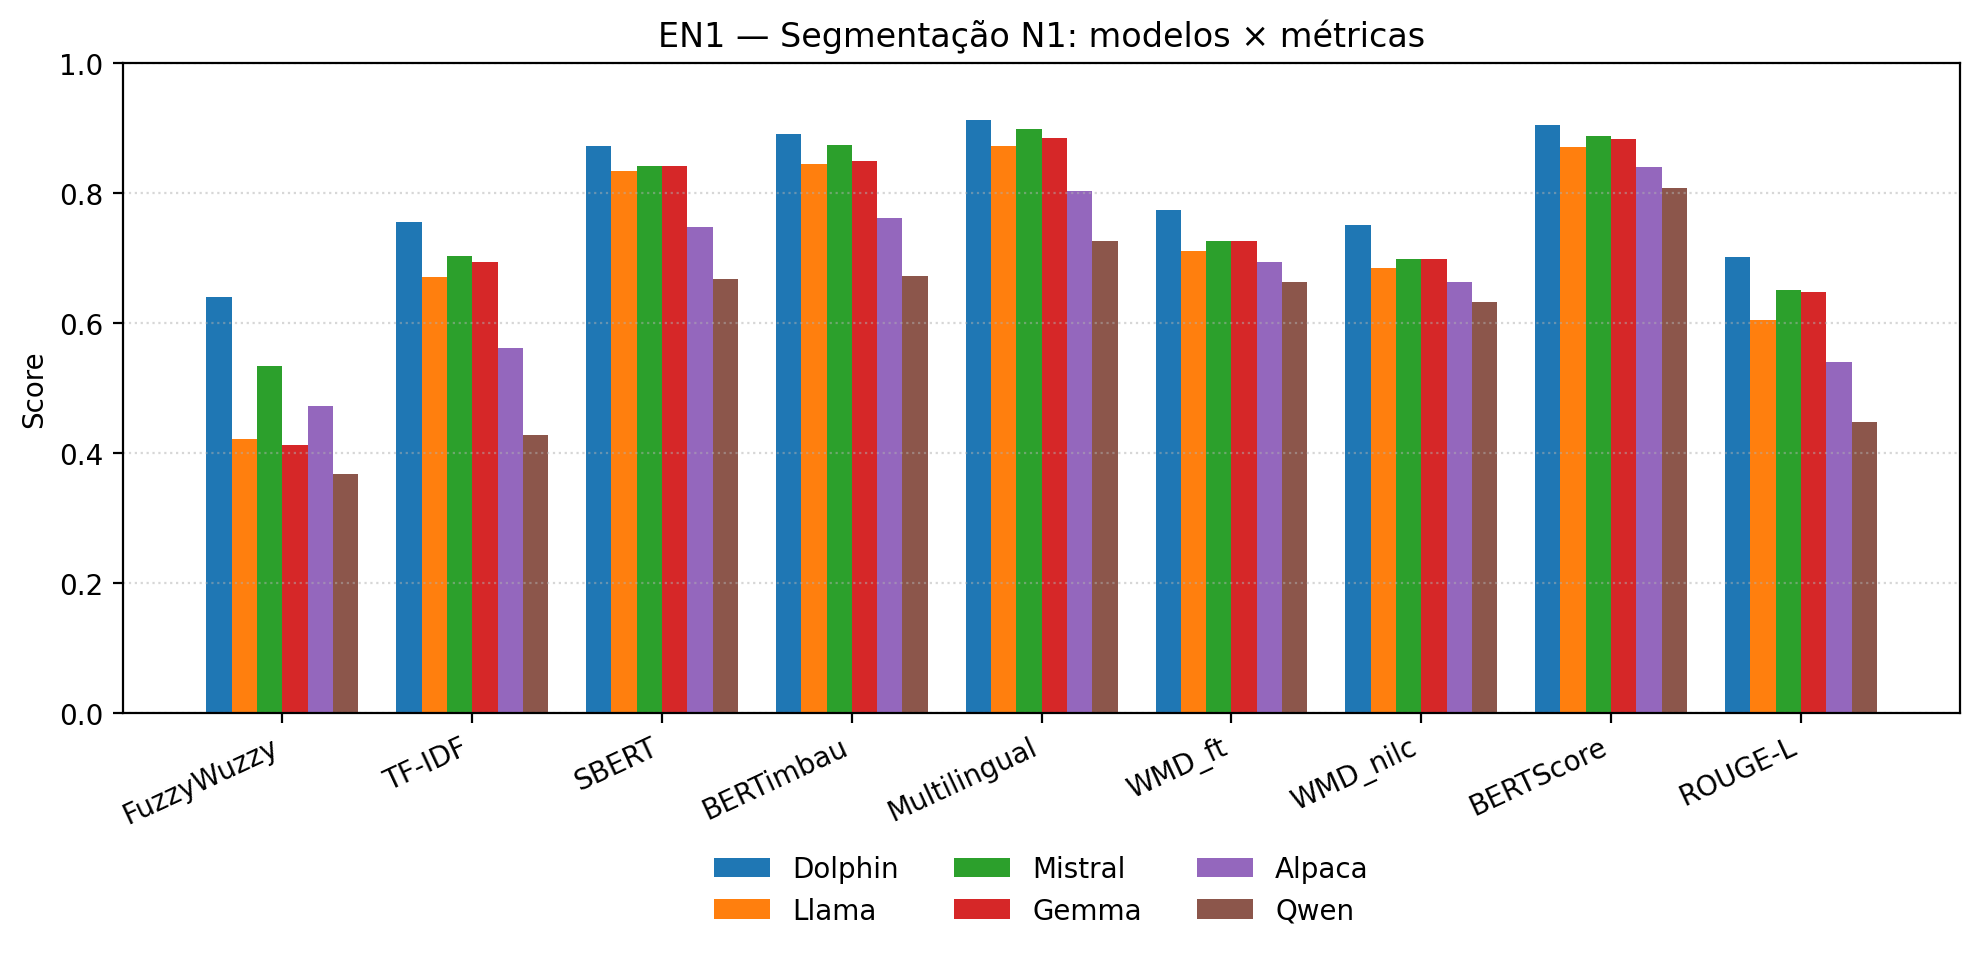
\includegraphics[width=0.95\linewidth]{figs/4.2.1-resultados-en1-barras.png}
\caption{Comparativo modelo $\times$ métrica em EN1.}
\label{img:4.2.1}
\end{figure}

\subsubsection{EN2: Identificação dos Operadores RASE}

O EN2 mediu a identificação e a estruturação dos operadores RASE a partir do N1 de referência. As médias caíram em relação ao EN1 (SBERT~0{,}490; Multilingual~0{,}595), o que reflete a maior dificuldade da formalização estruturada. As métricas de classificação caem ainda mais (F1 macro~0{,}197): os modelos têm dificuldade real em distinguir Seleção e Exceção. O \textbf{Llama} lidera nas métricas semânticas e lexicais; o \textbf{Dolphin} fica com a melhor F1 macro (0{,}286). Os números detalhados estão na Tabela~\ref{tab:resultados_en2}.

\begin{table}[ht]
\centering
\caption{Resultados por modelo em EN2 (similaridade e classificação macro por operador).}
\label{tab:resultados_en2}
\scriptsize
\begin{tabular}{lccccccccc}
\hline
 & \multicolumn{2}{c}{Lexical} & \multicolumn{3}{c}{Semântica} & \multicolumn{2}{c}{WMD} & \multicolumn{2}{c}{Geração} \\
\cline{2-3}\cline{4-6}\cline{7-8}\cline{9-10}
Modelo & FW & TF-IDF & SBERT & BERTimbau & Multi. & WMD\_ft & WMD\_nilc & BERTScore & ROUGE-L \\
\hline
Alpaca  & \pior{0{,}334} & 0{,}168 & 0{,}386 & 0{,}418 & 0{,}484 & 0{,}522 & 0{,}486 & \textbf{0{,}702} & 0{,}172 \\
Dolphin & 0{,}511 & 0{,}423 & 0{,}557 & 0{,}621 & 0{,}665 & \melhor{0{,}620} & \melhor{0{,}589} & \textbf{0{,}786} & 0{,}412 \\
Gemma   & 0{,}384 & 0{,}364 & 0{,}520 & 0{,}579 & 0{,}625 & 0{,}608 & 0{,}577 & \textbf{0{,}772} & 0{,}350 \\
Llama   & \melhor{0{,}638} & \melhor{0{,}447} & \melhor{0{,}595} & \melhor{0{,}657} & \melhor{0{,}685} & 0{,}617 & 0{,}586 & \melhor{\textbf{0{,}796}} & \melhor{0{,}427} \\
Mistral & 0{,}563 & 0{,}385 & 0{,}575 & 0{,}607 & 0{,}665 & 0{,}607 & 0{,}575 & \textbf{0{,}779} & 0{,}377 \\
Qwen    & 0{,}336 & \pior{0{,}083} & \pior{0{,}304} & \pior{0{,}369} & \pior{0{,}444} & \pior{0{,}496} & \pior{0{,}462} & \pior{0{,}684} & \pior{0{,}111} \\
\hline
\multicolumn{10}{@{}l}{\textit{Métricas de classificação} (macro por operador)} \\
Modelo  & \multicolumn{2}{c}{Acurácia} & \multicolumn{2}{c}{Precisão} & \multicolumn{2}{c}{Revocação} & \multicolumn{3}{c}{F1} \\
\hline
Alpaca  & \multicolumn{2}{c}{\pior{0{,}081}} & \multicolumn{2}{c}{0{,}103} & \multicolumn{2}{c}{0{,}109} & \multicolumn{3}{c}{0{,}105} \\
Dolphin & \multicolumn{2}{c}{0{,}339} & \multicolumn{2}{c}{\melhor{0{,}301}} & \multicolumn{2}{c}{0{,}276} & \multicolumn{3}{c}{\melhor{0{,}286}} \\
Gemma   & \multicolumn{2}{c}{0{,}182} & \multicolumn{2}{c}{0{,}252} & \multicolumn{2}{c}{\melhor{0{,}300}} & \multicolumn{3}{c}{0{,}265} \\
Llama   & \multicolumn{2}{c}{\melhor{0{,}439}} & \multicolumn{2}{c}{0{,}237} & \multicolumn{2}{c}{0{,}250} & \multicolumn{3}{c}{0{,}243} \\
Mistral & \multicolumn{2}{c}{0{,}434} & \multicolumn{2}{c}{0{,}268} & \multicolumn{2}{c}{0{,}214} & \multicolumn{3}{c}{0{,}238} \\
Qwen    & \multicolumn{2}{c}{0{,}160} & \multicolumn{2}{c}{\pior{0{,}051}} & \multicolumn{2}{c}{\pior{0{,}039}} & \multicolumn{3}{c}{\pior{0{,}044}} \\
\hline
\end{tabular}
\end{table}

A Figura~\ref{img:4.2.2} consolida o desempenho dos seis modelos nas nove métricas de similaridade em EN2.

\begin{figure}[ht]
\centering
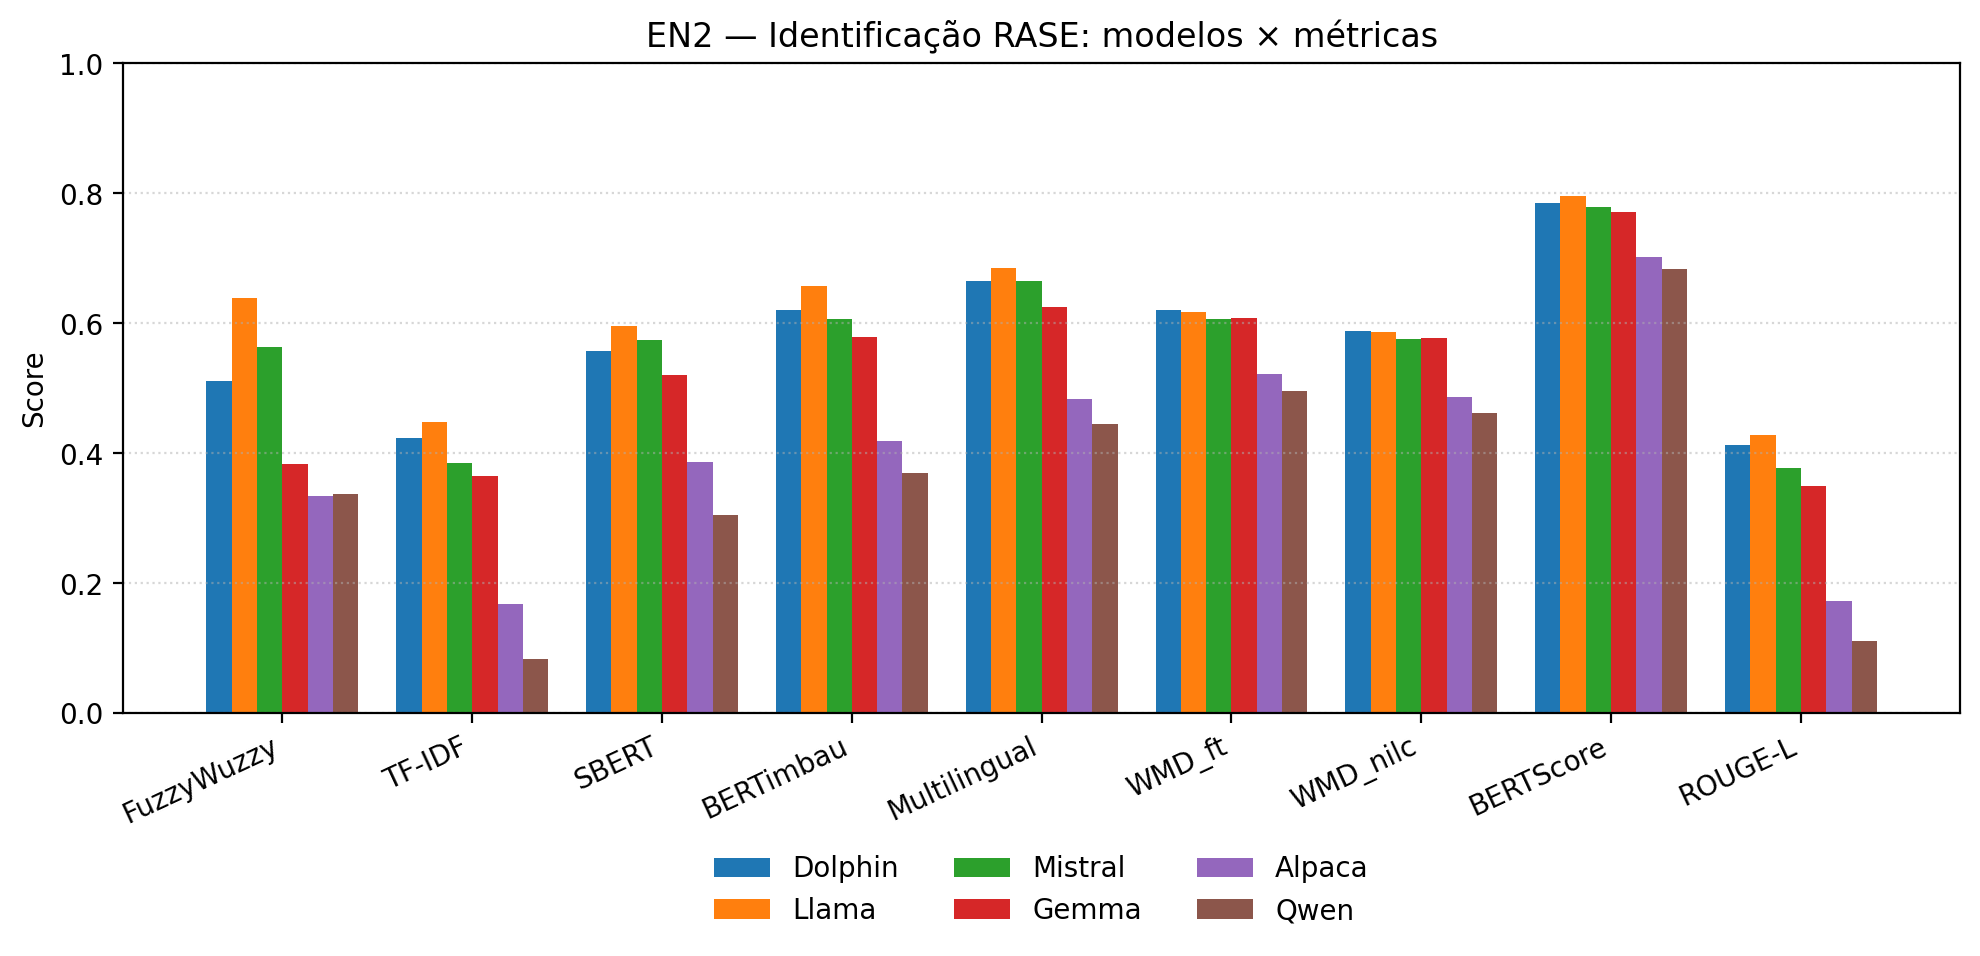
\includegraphics[width=0.95\linewidth]{figs/4.2.2-resultados-en2-barras.png}
\caption{Comparativo modelo $\times$ métrica em EN2.}
\label{img:4.2.2}
\end{figure}

\subsubsection{EN1N2: Pipeline Encadeado}

O EN1N2 testou a robustez do \textit{pipeline} totalmente automatizado: o N1 produzido pelo modelo na primeira etapa alimenta o N2 do mesmo modelo. Os resultados confirmam a hipótese de \textbf{propagação de erros}, mas com uma surpresa. As médias caem em relação ao EN2 em parte das métricas e se mantêm próximas ou até melhoram em outras, caso das semânticas: Multilingual sobe de 0{,}595 para 0{,}679; BERTimbau de 0{,}542 para 0{,}631; SBERT de 0{,}490 para 0{,}594. O motivo é que o \textit{pipeline} produz saídas mais próximas das frases originais e, por isso, mais alinhadas ao texto de referência no nível semântico, ainda que perca precisão na atribuição dos operadores. A liderança é compartilhada: o \textbf{Dolphin} domina TF-IDF, WMD\_ft, WMD\_nilc, BERTScore e ROUGE-L; o \textbf{Llama} lidera SBERT e empata em Multilingual. Os números completos estão na Tabela~\ref{tab:resultados_en1n2}.

\begin{table}[ht]
\centering
\caption{Resultados por modelo em EN1N2 (similaridade).}
\label{tab:resultados_en1n2}
\scriptsize
\begin{tabular}{lccccccccc}
\hline
 & \multicolumn{2}{c}{Lexical} & \multicolumn{3}{c}{Semântica} & \multicolumn{2}{c}{WMD} & \multicolumn{2}{c}{Geração} \\
\cline{2-3}\cline{4-6}\cline{7-8}\cline{9-10}
Modelo & FW & TF-IDF & SBERT & BERTimbau & Multi. & WMD\_ft & WMD\_nilc & BERTScore & ROUGE-L \\
\hline
Alpaca  & 0{,}375 & 0{,}285 & 0{,}494 & 0{,}523 & 0{,}581 & 0{,}573 & 0{,}538 & \textbf{0{,}742} & 0{,}282 \\
Dolphin & 0{,}549 & \melhor{0{,}529} & 0{,}662 & \textbf{0{,}711} & \melhor{\textbf{0{,}749}} & \melhor{0{,}673} & \melhor{0{,}644} & \melhor{\textbf{0{,}826}} & \melhor{0{,}509} \\
Gemma   & 0{,}391 & 0{,}458 & 0{,}615 & 0{,}656 & \textbf{0{,}701} & 0{,}646 & 0{,}617 & \textbf{0{,}804} & 0{,}436 \\
Llama   & \melhor{0{,}570} & 0{,}521 & \melhor{0{,}677} & \melhor{\textbf{0{,}721}} & \melhor{\textbf{0{,}749}} & 0{,}649 & 0{,}620 & \textbf{0{,}821} & 0{,}488 \\
Mistral & 0{,}559 & 0{,}489 & 0{,}667 & 0{,}698 & \textbf{0{,}740} & 0{,}648 & 0{,}618 & \textbf{0{,}817} & 0{,}468 \\
Qwen    & \pior{0{,}342} & \pior{0{,}219} & \pior{0{,}448} & \pior{0{,}478} & \pior{0{,}551} & \pior{0{,}562} & \pior{0{,}530} & \pior{\textbf{0{,}731}} & \pior{0{,}240} \\
\hline
\end{tabular}
\end{table}

A Figura~\ref{img:4.2.3} apresenta o comparativo visual em EN1N2, evidenciando a alternância de liderança entre Dolphin e Llama por métrica.

\begin{figure}[ht]
\centering
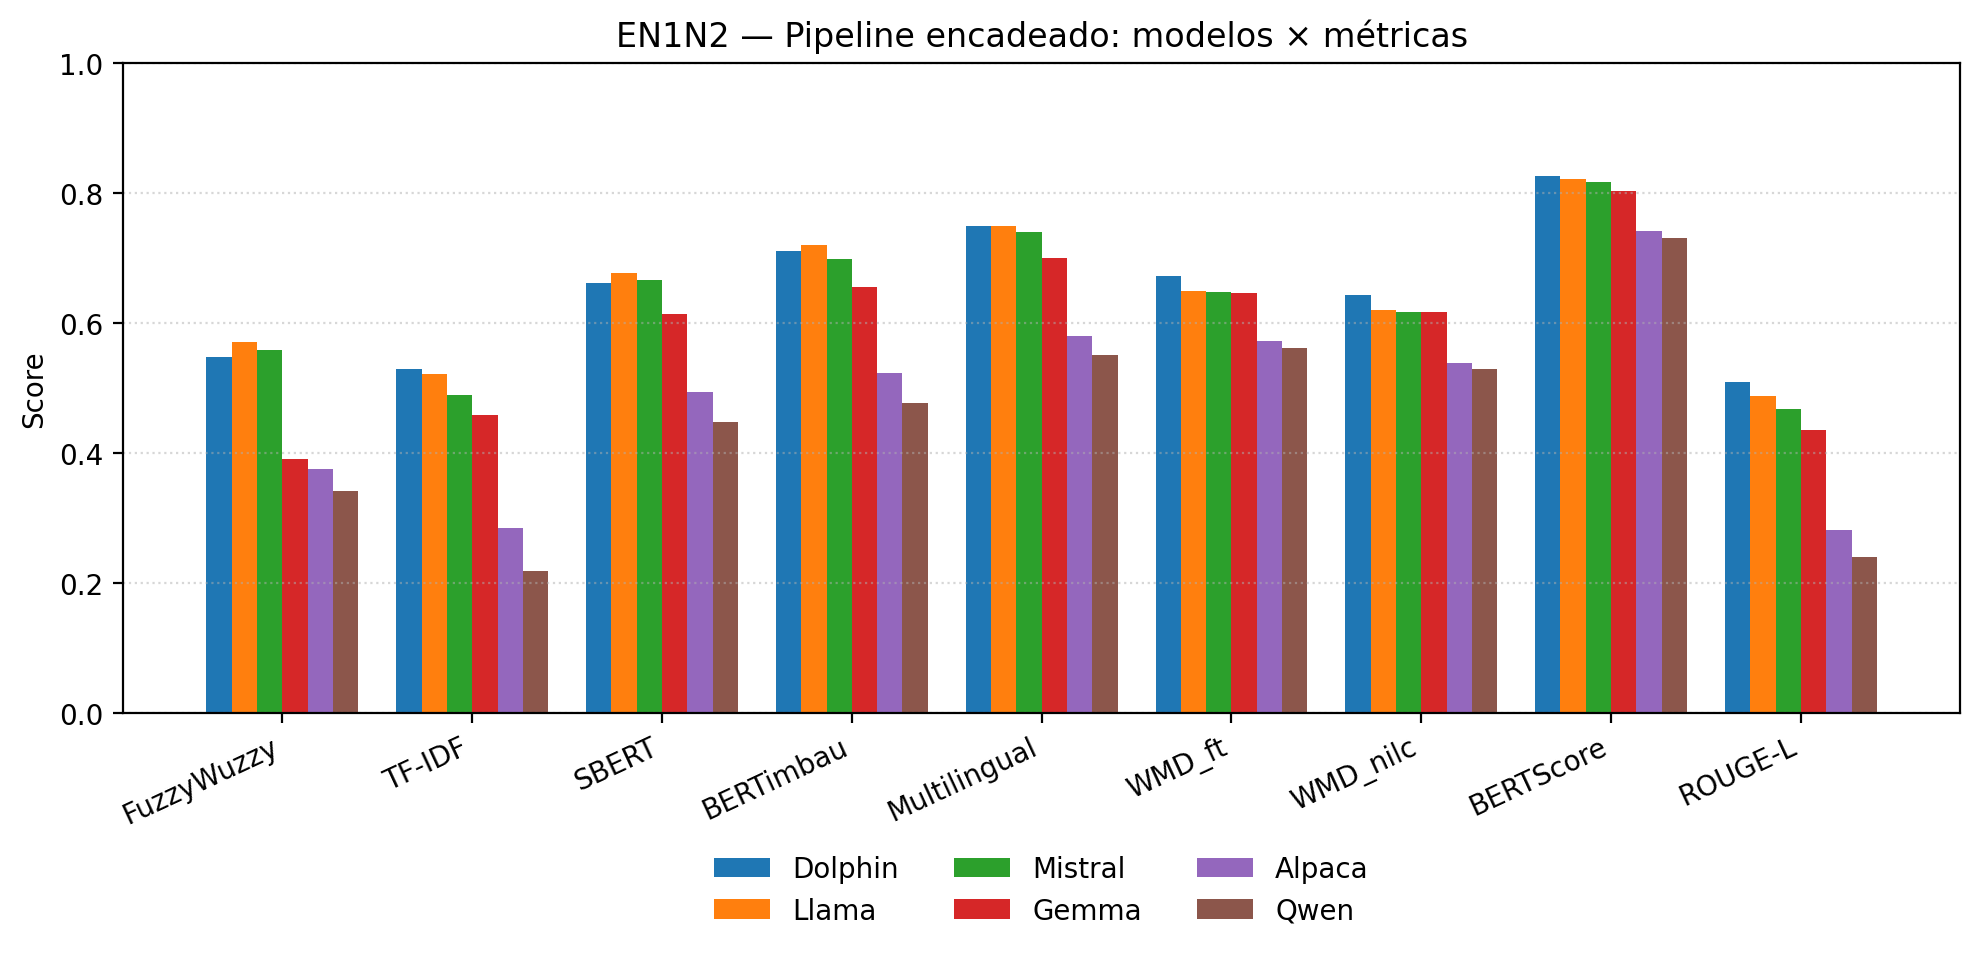
\includegraphics[width=0.95\linewidth]{figs/4.2.3-resultados-en1n2-barras.png}
\caption{Comparativo modelo $\times$ métrica em EN1N2.}
\label{img:4.2.3}
\end{figure}

\subsubsection{EN3: Estruturação Semântica em JSON com N2 de referência}

O nível N3 (estruturação semântica em JSON) foi avaliado em dois cenários complementares: o EN3, em isolamento, recebendo como entrada os operadores N2 de referência; e o EN1N2N3, no \textit{pipeline} encadeado de ponta a ponta, em que o N1 gerado alimenta o N2 do mesmo modelo, que por sua vez alimenta o N3 do mesmo modelo. Em ambos os cenários, a comparação não é entre \textit{strings} normativas inteiras, e sim campo a campo (\texttt{type}, \texttt{object}, \texttt{property}, \texttt{comparation}, \texttt{target} e \texttt{unit}), sobre a serialização canônica do JSON gerado contra o JSON anotado.

Como a saída é \textit{quase-estruturada} e composta por campos curtos com vocabulário restrito, as métricas de similaridade textual sobem para patamares bem mais altos do que em N1 e N2 (ver Tabela~\ref{tab:resultados_n3}). As métricas de classificação por correspondência exata, em compensação, mostram um quadro bem mais duro: a precisão macro fica abaixo de 4\%. Isso sinaliza que os modelos preservam o significado, mas variam o vocabulário em relação à referência, por exemplo \texttt{target = ``público''} em vez de \texttt{target = ``uso público''}. O \textbf{Llama} dominou: liderou em \textit{todas} as nove métricas de similaridade, com SBERT~0{,}947 e Multilingual~0{,}928. Mistral, Dolphin e Qwen ficam próximos em métricas semânticas, mostrando que a etapa N3 isolada é a mais homogênea entre os modelos avaliados.

\begin{table}[ht]
\centering
\caption{Resultados por modelo em EN3 (similaridade e classificação macro por campo).}
\label{tab:resultados_n3}
\scriptsize
\begin{tabular}{lccccccccc}
\hline
 & \multicolumn{2}{c}{Lexical} & \multicolumn{3}{c}{Semântica} & \multicolumn{2}{c}{WMD} & \multicolumn{2}{c}{Geração} \\
\cline{2-3}\cline{4-6}\cline{7-8}\cline{9-10}
Modelo & FW & TF-IDF & SBERT & BERTimbau & Multi. & WMD\_ft & WMD\_nilc & BERTScore & ROUGE-L \\
\hline
Alpaca  & \pior{\textbf{0{,}729}} & \pior{0{,}395} & \pior{\textbf{0{,}846}} & \pior{\textbf{0{,}745}} & \pior{\textbf{0{,}798}} & \pior{\textbf{0{,}756}} & \pior{\textbf{0{,}751}} & \textbf{0{,}815} & \pior{0{,}624} \\
Dolphin & \textbf{0{,}860} & 0{,}694 & \textbf{0{,}912} & \textbf{0{,}848} & \textbf{0{,}887} & \textbf{0{,}842} & \textbf{0{,}839} & \textbf{0{,}901} & \textbf{0{,}799} \\
Gemma   & \textbf{0{,}751} & 0{,}480 & \textbf{0{,}858} & \textbf{0{,}755} & \textbf{0{,}823} & \textbf{0{,}762} & \textbf{0{,}757} & \pior{\textbf{0{,}810}} & 0{,}652 \\
Llama   & \melhor{\textbf{0{,}892}} & \melhor{\textbf{0{,}736}} & \melhor{\textbf{0{,}947}} & \melhor{\textbf{0{,}897}} & \melhor{\textbf{0{,}928}} & \melhor{\textbf{0{,}915}} & \melhor{\textbf{0{,}912}} & \melhor{\textbf{0{,}925}} & \melhor{\textbf{0{,}871}} \\
Mistral & \textbf{0{,}877} & 0{,}689 & \textbf{0{,}938} & \textbf{0{,}891} & \textbf{0{,}914} & \textbf{0{,}903} & \textbf{0{,}900} & \textbf{0{,}922} & \textbf{0{,}842} \\
Qwen    & \textbf{0{,}872} & 0{,}590 & \textbf{0{,}937} & \textbf{0{,}877} & \textbf{0{,}889} & \textbf{0{,}898} & \textbf{0{,}895} & \textbf{0{,}905} & \textbf{0{,}804} \\
\hline
\multicolumn{10}{@{}l}{\textit{Métricas de classificação} (macro por campo)} \\
Modelo  & \multicolumn{2}{c}{Acurácia} & \multicolumn{2}{c}{Precisão} & \multicolumn{2}{c}{Revocação} & \multicolumn{3}{c}{F1} \\
\hline
Alpaca  & \multicolumn{2}{c}{\pior{0{,}283}} & \multicolumn{2}{c}{0{,}012} & \multicolumn{2}{c}{0{,}434} & \multicolumn{3}{c}{0{,}024} \\
Dolphin & \multicolumn{2}{c}{\textbf{0{,}705}} & \multicolumn{2}{c}{0{,}034} & \multicolumn{2}{c}{0{,}447} & \multicolumn{3}{c}{0{,}062} \\
Gemma   & \multicolumn{2}{c}{0{,}292} & \multicolumn{2}{c}{0{,}017} & \multicolumn{2}{c}{\melhor{0{,}603}} & \multicolumn{3}{c}{0{,}033} \\
Llama   & \multicolumn{2}{c}{\textbf{0{,}725}} & \multicolumn{2}{c}{\melhor{0{,}038}} & \multicolumn{2}{c}{0{,}361} & \multicolumn{3}{c}{\melhor{0{,}067}} \\
Mistral & \multicolumn{2}{c}{\melhor{\textbf{0{,}760}}} & \multicolumn{2}{c}{0{,}037} & \multicolumn{2}{c}{0{,}371} & \multicolumn{3}{c}{0{,}066} \\
Qwen    & \multicolumn{2}{c}{0{,}692} & \multicolumn{2}{c}{\pior{0{,}004}} & \multicolumn{2}{c}{\pior{0{,}063}} & \multicolumn{3}{c}{\pior{0{,}008}} \\
\hline
\end{tabular}
\end{table}

O setup foi idêntico ao dos experimentos anteriores: os mesmos seis LLMs servidos via Ollama, os mesmos \textit{prompts} \textit{few-shot} por operador, o mesmo \textit{dataset} de 79 normas. Saídas por modelo ficam em arquivos JSON dedicados (\texttt{generate\_n3\_<modelo>.json}); o agregado vive em um único arquivo de métricas (\texttt{validate\_n3.json}). A correspondência exata por campo é mais dura que o limiar de similaridade adotado em N1 e N2, o que derruba a precisão observada, em especial nos modelos com menor aderência ao esquema (Alpaca e Qwen).

\subsubsection{EN1N2N3: Pipeline Encadeado Completo}

O EN1N2N3 é o \textit{pipeline} automatizado de ponta a ponta. Este é o cenário que replica o uso real em produção: a única entrada é o texto bruto da norma, e a saída final é o JSON estruturado por operador. Como cada etapa acumula transformações, é também o experimento mais sujeito à \textbf{propagação de erros}: as médias caem em relação ao EN3 isolado em todas as métricas (SBERT~0{,}777 \textit{vs.}~0{,}906; Multilingual~0{,}793 \textit{vs.}~0{,}873; BERTScore~0{,}843 \textit{vs.}~0{,}880). Ainda assim, os patamares absolutos permanecem superiores aos observados em EN2 e EN1N2, beneficiados pelo vocabulário restrito do JSON. A Tabela~\ref{tab:resultados_en1n2n3} traz os resultados por modelo.

\begin{table}[ht]
\centering
\caption{Resultados por modelo em EN1N2N3 (similaridade sobre o JSON estruturado).}
\label{tab:resultados_en1n2n3}
\scriptsize
\begin{tabular}{lccccccccc}
\hline
 & \multicolumn{2}{c}{Lexical} & \multicolumn{3}{c}{Semântica} & \multicolumn{2}{c}{WMD} & \multicolumn{2}{c}{Geração} \\
\cline{2-3}\cline{4-6}\cline{7-8}\cline{9-10}
Modelo & FW & TF-IDF & SBERT & BERTimbau & Multi. & WMD\_ft & WMD\_nilc & BERTScore & ROUGE-L \\
\hline
Alpaca  & \pior{0{,}525} & \pior{0{,}345} & \pior{0{,}687} & \pior{0{,}645} & \pior{\textbf{0{,}701}} & \pior{0{,}676} & \pior{0{,}658} & \pior{\textbf{0{,}782}} & \pior{0{,}471} \\
Dolphin & 0{,}685 & 0{,}600 & \textbf{0{,}811} & \textbf{0{,}794} & \textbf{0{,}832} & \textbf{0{,}776} & \textbf{0{,}762} & \textbf{0{,}871} & 0{,}683 \\
Gemma   & 0{,}536 & 0{,}419 & \textbf{0{,}747} & \textbf{0{,}710} & \textbf{0{,}767} & \textbf{0{,}712} & 0{,}697 & \textbf{0{,}807} & 0{,}553 \\
Llama   & \melhor{\textbf{0{,}701}} & \melhor{0{,}630} & \melhor{\textbf{0{,}834}} & \melhor{\textbf{0{,}823}} & \melhor{\textbf{0{,}853}} & \melhor{\textbf{0{,}804}} & \melhor{\textbf{0{,}790}} & \melhor{\textbf{0{,}882}} & \melhor{\textbf{0{,}711}} \\
Mistral & 0{,}693 & 0{,}600 & \textbf{0{,}830} & \textbf{0{,}814} & \textbf{0{,}845} & \textbf{0{,}801} & \textbf{0{,}788} & \textbf{0{,}879} & 0{,}691 \\
Qwen    & 0{,}561 & 0{,}490 & \textbf{0{,}750} & \textbf{0{,}724} & \textbf{0{,}762} & \textbf{0{,}773} & \textbf{0{,}759} & \textbf{0{,}838} & 0{,}590 \\
\hline
\end{tabular}
\end{table}

A saída de cada modelo é persistida em um arquivo JSON próprio (\textit{generate\_n1n2n3\_<modelo>.json}), e as métricas agregadas ficam em um arquivo único (\textit{validate\_n1n2n3.json}). O \textbf{Llama} mantém a liderança que conquistou em EN3 isolado, agora em todas as nove métricas de similaridade; \textbf{Mistral} fica imediatamente atrás, com diferenças marginais (Multilingual~0{,}845 \textit{vs.}~0{,}853). Em linha com o padrão observado em EN1N2, Llama, Mistral e Dolphin preservam vantagem relativa também na cadeia completa, ao passo que Alpaca e Gemma acumulam queda em todas as métricas e entregam o pior desempenho global, evidenciando que falhas em N1/N2 contaminam a estruturação final em N3 mesmo nas métricas semânticas.

\subsection{Resultados por Modelo}

A Tabela~\ref{tab:ranking_global} traz a média global por modelo, agregando as nove métricas de similaridade textual sobre os cinco experimentos (EN1, EN2, EN1N2, EN3 e EN1N2N3). O ranking final foge do esperado: o líder é o \textbf{Llama}, sustentado pela liderança absoluta em EN3 e EN1N2N3 (ambas as etapas N3) e pelo melhor desempenho em EN2. O \textbf{Dolphin} fica em segundo: domina o EN1 com folga e mantém desempenho competitivo nas etapas seguintes. Mistral aparece em terceiro, seguido por Gemma, Qwen e Alpaca.

\begin{table}[ht]
\centering
\caption{Média global por modelo (nove métricas de similaridade $\times$ cinco experimentos).}
\label{tab:ranking_global}
\small
\begin{tabular}{lcccccc}
\hline
Modelo  & EN1   & EN2   & EN1N2 & EN3   & EN1N2N3 & Média Global \\
\hline
Llama   & \textbf{0{,}724} & \melhor{0{,}605} & 0{,}646 & \melhor{\textbf{0{,}892}} & \melhor{\textbf{0{,}781}} & \melhor{\textbf{0{,}730}} \\
Dolphin & \melhor{\textbf{0{,}801}} & 0{,}576 & \melhor{0{,}650} & \textbf{0{,}843} & \textbf{0{,}757} & \textbf{0{,}725} \\
Mistral & \textbf{0{,}757} & 0{,}570 & 0{,}634 & \textbf{0{,}875} & \textbf{0{,}771} & \textbf{0{,}721} \\
Gemma   & \textbf{0{,}738} & 0{,}531 & 0{,}591 & \textbf{0{,}739} & 0{,}661 & 0{,}652 \\
Qwen    & \pior{0{,}602} & \pior{0{,}366} & \pior{0{,}456} & \textbf{0{,}852} & 0{,}694 & 0{,}594 \\
Alpaca  & 0{,}676 & 0{,}408 & 0{,}488 & \pior{\textbf{0{,}718}} & \pior{0{,}610} & \pior{0{,}580} \\
\hline
\end{tabular}
\end{table}

A seguir, destacam-se as observações por modelo.

\textbf{Llama.} Lidera a média global (0{,}730) e domina os experimentos do nível N3: em EN3 isolado ficou à frente em \textit{todas} as nove métricas (SBERT~0{,}947; Multilingual~0{,}928; BERTScore~0{,}925); em EN1N2N3, repetiu a liderança nas nove métricas (SBERT~0{,}834; Multilingual~0{,}853; BERTScore~0{,}882). Foi também o melhor em EN2 em sete métricas: FuzzyWuzzy (0{,}638), TF-IDF (0{,}447), SBERT (0{,}595), BERTimbau (0{,}657), Multilingual (0{,}685), BERTScore (0{,}796) e ROUGE-L (0{,}427), além da maior acurácia macro de classificação no mesmo experimento (0{,}439). No EN1N2, liderou em FuzzyWuzzy (0{,}570), SBERT (0{,}677) e BERTimbau (0{,}721), empatando com o Dolphin em Multilingual (0{,}749). É a escolha quando se tolera o custo computacional.

\textbf{Dolphin.} Foi o melhor segmentador em EN1, com domínio absoluto nas nove métricas (BERTimbau~0{,}891; Multilingual~0{,}913; SBERT~0{,}873; BERTScore~0{,}905) e a melhor F1 macro de classificação no experimento (0{,}806). No EN2, liderou em WMD\_ft (0{,}620), WMD\_nilc (0{,}589) e F1 macro (0{,}286). No EN1N2, ficou à frente em TF-IDF (0{,}529), WMD\_ft (0{,}673), WMD\_nilc (0{,}644), BERTScore (0{,}826) e ROUGE-L (0{,}509). Em EN3 e EN1N2N3, mantém desempenho competitivo (SBERT~0{,}912 e 0{,}811, respectivamente), embora atrás de Llama e Mistral. Soma-se a isso o baixo custo computacional (Seção~\ref{sec:tempo}), o que rende a melhor relação custo-benefício observada.

\textbf{Mistral.} Desempenho consistente em todos os cenários, e o mais regular da bateria: terceiro colocado na média global (0{,}721), a menos de um ponto percentual do líder. Ficou próximo dos líderes em EN1 (Multilingual~0{,}899; BERTimbau~0{,}874) e em EN1N2 (Multilingual~0{,}740; BERTimbau~0{,}698), entregou a segunda melhor acurácia macro do EN2 (0{,}434), e fica colado ao Llama em EN3 (SBERT~0{,}938) e em EN1N2N3 (SBERT~0{,}830).

\textbf{Gemma.} Aparece como líder em revocação macro de classificação tanto no EN1 (0{,}917) quanto no EN2 (0{,}300), ou seja, boa cobertura, com precisão menor. As médias semânticas ficam em patamar intermediário.

\textbf{Alpaca.} Desempenho fraco em todos os experimentos, com queda acentuada no EN2 (SBERT~0{,}386; F1 macro~0{,}105).

\textbf{Qwen.} Pior desempenho geral. Colapsou no EN2 (TF-IDF~0{,}083; F1 macro~0{,}044) e teve a maior latência do \textit{pipeline} encadeado (ver Seção~\ref{sec:tempo}). Pesa também a tendência do modelo a gerar saídas em chinês simplificado, fora do idioma esperado.

\subsection{Análise por Métrica}

\textbf{Métricas lexicais.} FuzzyWuzzy e TF-IDF caem claramente de EN1 para EN2 (FuzzyWuzzy: 0{,}475 $\rightarrow$ 0{,}461; TF-IDF: 0{,}636 $\rightarrow$ 0{,}312). Como dependem de sobreposição lexical, essas métricas punem as reformulações sintáticas e as sinonímias geradas pelos LLMs. Em EN3 e EN1N2N3, voltam a subir (FuzzyWuzzy: 0{,}847 e 0{,}617; TF-IDF: 0{,}597 e 0{,}514), beneficiadas pelo vocabulário curto e restrito do JSON.

\textbf{Métricas semânticas.} SBERT, BERTimbau e Multilingual mantêm médias altas e estáveis. O BERTimbau, treinado sobre texto jurídico em português, fica ligeiramente acima do SBERT em quase todos os modelos e experimentos (EN1: 0{,}816 \textit{vs.}~0{,}801; EN1N2: 0{,}631 \textit{vs.}~0{,}594), evidência prática do ganho de usar \textit{embeddings} de domínio para validar transformações normativas. Em EN3, atingem os valores mais altos da bateria (SBERT~0{,}906; Multilingual~0{,}873), porque os campos JSON contêm sintagmas curtos com baixa variação léxica.

\textbf{Métricas voltadas para geração.} O BERTScore teve a maior média absoluta em EN2 (0{,}753) e em EN1N2 (0{,}790), graças ao alinhamento ótimo entre \textit{tokens} mesmo quando há forte reformulação. Em EN3 e EN1N2N3, segue alto (0{,}880 e 0{,}843). Já o ROUGE-L comportou-se como métrica lexical, com queda acentuada em EN2 (0{,}308) e recuperação em EN3 (0{,}765).

\textbf{Métricas de distância (WMD).} Desempenho intermediário, entre lexicais e semânticas. Os valores foram mais altos em EN1 (WMD\_ft~0{,}716; WMD\_nilc~0{,}688) e em EN3 (WMD\_ft~0{,}846; WMD\_nilc~0{,}842), refletindo a proximidade lexical maior entre as saídas e o texto/JSON de referência nesses dois cenários.

\textbf{Métricas de classificação.} Em EN1, a F1 macro chega a 0{,}806 (Dolphin), o que indica que a maior parte das sentenças atômicas é segmentada corretamente. Em EN2, a F1 desaba para 0{,}286 no melhor caso (Dolphin), com colapso em Seleção e Exceção: F1 próxima de zero para todos os modelos. Esses dois operadores são especialmente difíceis de identificar mesmo para os líderes. Em EN3, a baixa precisão por correspondência exata (precisão macro abaixo de 4\% para todos os modelos) mostra que o emparelhamento \textit{token} a \textit{token} é severo demais para um campo cuja semântica resiste a variações léxicas legítimas.

\subsection{Tempo de Execução}
\label{sec:tempo}

O tempo total de geração foi medido por modelo e por experimento. A Tabela~\ref{tab:tempo_n1} traz os tempos em N1; a Tabela~\ref{tab:tempo_n2}, em N2; a Tabela~\ref{tab:tempo_n1n2}, no \textit{pipeline} encadeado N1N2; a Tabela~\ref{tab:tempo_n3} traz os tempos do EN3 (N3 isolado, com N2 de referência como entrada); e a Tabela~\ref{tab:tempo_n1n2n3}, do \textit{pipeline} completo EN1N2N3.

\begin{table}[ht]
\centering
\caption{Tempo total de geração por modelo em N1.}
\label{tab:tempo_n1}
\begin{tabular}{lrr}
\hline
Modelo & Tempo (s) & Tempo (h:mm:ss) \\
\hline
Alpaca  & 104{,}55 & 0:01:44 \\
Dolphin & \melhor{62{,}65} & \melhor{0:01:02} \\
Gemma   & 133{,}04 & 0:02:13 \\
Llama   & \pior{5\,676{,}97} & \pior{1:34:36} \\
Mistral & 70{,}04 & 0:01:10 \\
Qwen    & 309{,}59 & 0:05:09 \\
\hline
\end{tabular}
\end{table}

\begin{table}[ht]
\centering
\caption{Tempo total de geração por modelo em N2.}
\label{tab:tempo_n2}
\begin{tabular}{lrr}
\hline
Modelo & Tempo (s) & Tempo (h:mm:ss) \\
\hline
Alpaca  & 249{,}10 & 0:04:09 \\
Dolphin & 124{,}69 & 0:02:04 \\
Gemma   & 244{,}19 & 0:04:04 \\
Llama   & \pior{6\,895{,}71} & \pior{1:54:55} \\
Mistral & \melhor{123{,}63} & \melhor{0:02:03} \\
Qwen    & 6\,515{,}09 & 1:48:35 \\
\hline
\end{tabular}
\end{table}

\begin{table}[ht]
\centering
\caption{Tempo total de geração por modelo em N1N2.}
\label{tab:tempo_n1n2}
\begin{tabular}{lrr}
\hline
Modelo & Tempo (s) & Tempo (h:mm:ss) \\
\hline
Alpaca  & 330{,}84 & 0:05:30 \\
Dolphin & \melhor{104{,}28} & \melhor{0:01:44} \\
Gemma   & 427{,}22 & 0:07:07 \\
Llama   & 9\,450{,}14 & 2:37:30 \\
Mistral & 138{,}39 & 0:02:18 \\
Qwen    & \pior{10\,093{,}84} & \pior{2:48:13} \\
\hline
\end{tabular}
\end{table}

\begin{table}[ht]
\centering
\caption{Tempo total de geração por modelo em N3 (EN3 isolado).}
\label{tab:tempo_n3}
\begin{tabular}{lrr}
\hline
Modelo & Tempo (s) & Tempo (h:mm:ss) \\
\hline
Alpaca  & 2\,104{,}92 & 0:35:05 \\
Dolphin & \melhor{584{,}96} & \melhor{0:09:45} \\
Gemma   & \pior{5\,982{,}38} & \pior{1:39:42} \\
Llama   & 800{,}78 & 0:13:21 \\
Mistral & 627{,}68 & 0:10:28 \\
Qwen    & 847{,}41 & 0:14:07 \\
\hline
\end{tabular}
\end{table}

\begin{table}[ht]
\centering
\caption{Tempo total de geração por modelo em N1N2N3 (\textit{pipeline} completo).}
\label{tab:tempo_n1n2n3}
\begin{tabular}{lrr}
\hline
Modelo & Tempo (s) & Tempo (h:mm:ss) \\
\hline
Alpaca  & 1\,395{,}35 & 0:23:15 \\
Dolphin & 757{,}65 & 0:12:38 \\
Gemma   & \pior{6\,364{,}48} & \pior{1:46:04} \\
Llama   & 808{,}62 & 0:13:29 \\
Mistral & \melhor{637{,}88} & \melhor{0:10:38} \\
Qwen    & 808{,}72 & 0:13:29 \\
\hline
\end{tabular}
\end{table}

Os tempos expõem um \textit{trade-off} nítido entre qualidade e custo computacional. Em EN1 e EN1N2, Llama e Qwen são os mais lentos: respectivamente 1h34min e 5min em N1; 2h37min e 2h48min em N1N2. Em EN3 e EN1N2N3, o quadro se inverte: o \textbf{Gemma} passa a ser o mais oneroso (1h39min em N3; 1h46min em N1N2N3), enquanto Llama, Mistral e Qwen ficam em torno de 10 a 14 minutos. O Dolphin combina alta qualidade com tempos na casa de 1 a 13 minutos em todos os experimentos (62~s em N1; 1m44s em N1N2; 9m45s em N3; 12m38s em N1N2N3), e segue como a melhor relação custo-benefício observada na bateria.

\subsection{Discussão Integrada}

A leitura conjunta dos três experimentos e das treze métricas permite consolidar cinco observações.

\textbf{1. \textit{Embeddings} semânticos e BERTScore são as métricas mais adequadas a esta tarefa.} SBERT, BERTimbau, Multilingual e BERTScore capturam equivalência mesmo quando há reformulação lexical pesada, e são as métricas mais estáveis ao longo dos experimentos. O BERTimbau, treinado em corpus jurídico em PT-BR, fica ligeiramente acima do SBERT, evidência do ganho de \textit{embeddings} de domínio.

\textbf{2. O \textit{pipeline} encadeado não degrada todas as métricas de forma uniforme.} A queda esperada pela propagação de erros aparece nas lexicais (FuzzyWuzzy, TF-IDF e ROUGE-L). Já nas semânticas, o EN1N2 chega a \textit{superar} o EN2 isolado nas médias agregadas (Multilingual~0{,}679 \textit{vs.}~0{,}595): o N1 produzido pelo próprio modelo tende a gerar frases próximas das originais, o que favorece o emparelhamento semântico, mesmo quando o N2 erra na atribuição dos operadores. As métricas de classificação confirmam, porém, que esse ganho não se converte em classificação RASE melhor: o \textit{pipeline} continua dependendo de saída atomizada e corretamente rotulada para que a verificação automática faça sentido.

\textbf{3. Há perfis complementares entre os modelos líderes.} O Llama lidera a qualidade global (0{,}730), com domínio absoluto sobre o nível N3 (as nove métricas em EN3 e em EN1N2N3) e também sobre o EN2; é a escolha quando se tolera o custo computacional. O Dolphin (0{,}725) entrega o melhor custo-benefício: domina o EN1, fica à frente nas métricas de distância do EN1N2 e tem o menor tempo de geração entre os líderes. O Mistral (0{,}721) é o terceiro e o mais consistente: nunca lidera com folga, mas nunca está longe.

\textbf{4. Qwen e Alpaca não são recomendados.} Ambos têm desempenho consistentemente inferior em todas as métricas e experimentos. O Qwen ainda registra a maior latência do \textit{pipeline} encadeado (2h48min) e tende a gerar saídas fora do idioma esperado.

\textbf{5. A decomposição em três níveis foi decisiva.} Separar segmentação (N1), classificação RASE (N2) e estruturação JSON (N3) viabilizou saídas válidas sem utilizar \textit{Fine-Tuning} nem \textit{Retrieval-Augmented Generation}, ou seja, Engenharia de Prompt sozinha basta para alcançar similaridade semântica perto de 0{,}90 nos melhores cenários (Dolphin em EN1, com BERTimbau~0{,}891; Llama em N3 isolado, com SBERT~0{,}947). O que sobra de dificuldade está concentrado na classificação correta dos operadores Seleção e Exceção em N2, as classes mais difíceis para todos os modelos avaliados.

\section{Conclusão}\label{sec:conclusao}

Este trabalho investigou a aplicação de seis LLMs \textit{open-source} (Llama, Dolphin, Gemma, Mistral, Alpaca e Qwen) na conversão automática de normas técnicas brasileiras da AEC para o formato RASE, usando \textbf{apenas Engenharia de Prompt}. A tarefa foi decomposta em três níveis sucessivos de normalização (N1, N2 e N3) e avaliada em cinco experimentos (EN1, EN2, EN1N2, EN3 e EN1N2N3), sobre um \textit{dataset} de 79 normas anotadas. A avaliação combinou treze métricas: nove de similaridade textual (lexicais, semânticas, de distância e voltadas para geração) e quatro de classificação, derivadas da matriz de confusão.

\subsection{Síntese dos Resultados}

A decomposição em três níveis viabilizou a conversão de normas AEC em representações RASE sem recorrer a \textit{Fine-Tuning} nem a \textit{Retrieval-Augmented Generation}. Engenharia de Prompt sozinha bastou para alcançar similaridade semântica perto de 0{,}90 nos melhores cenários (Dolphin em EN1, com BERTimbau~0{,}891 e Multilingual~0{,}913; Llama em EN3 isolado, com SBERT~0{,}947; e novamente Llama em EN1N2N3, com SBERT~0{,}834 mesmo na cadeia completa). As métricas baseadas em \textit{embeddings} (SBERT, BERTimbau, Multilingual) e o BERTScore foram as mais adequadas para validar transformações normativas, porque toleram reformulações que preservam o sentido. O BERTimbau manteve ganho consistente sobre o SBERT, evidência prática do valor de \textit{embeddings} de domínio jurídico em PT-BR.

No agregado das nove métricas de similaridade sobre os cinco experimentos, o \textbf{Llama} fechou com a melhor média global (0{,}730), puxado pela liderança absoluta em EN3 e EN1N2N3 (as duas etapas do nível N3) e em EN2. O \textbf{Dolphin} ficou em segundo (0{,}725), com a melhor relação custo-benefício: cerca de noventa vezes mais rápido que o Llama no \textit{pipeline} encadeado, e líder absoluto em EN1. O Mistral fechou em terceiro (0{,}721), o mais consistente da bateria. Qwen e Alpaca apresentaram desempenho insatisfatório nas etapas mais sensíveis a falhas semânticas (EN2 e EN1N2), mas se recuperaram em EN3, beneficiados pelo vocabulário restrito do JSON. As métricas de classificação confirmaram um achado importante: os operadores Seleção e Exceção são as classes mais difíceis em N2 para todos os modelos, com F1 próxima de zero; já em EN3, a correspondência exata por campo derruba a precisão macro para abaixo de 4\%, apontando a necessidade de critérios de classificação mais flexíveis para o nível N3.

\subsection{Contribuições}

A pesquisa entrega cinco contribuições centrais:

\begin{itemize}
    \item A definição operacional de três níveis de normalização sobre a metodologia RASE: \textbf{N1} (segmentação atômica), \textbf{N2} (identificação dos operadores RASE) e \textbf{N3} (estruturação semântica em JSON), com \textit{prompts} dedicados a cada nível e a cada operador.
    \item Uma comparação sistemática de seis LLMs \textit{open-source} servidos localmente via Ollama, na tarefa de conversão de normas brasileiras da AEC, sob protocolo experimental idêntico (mesmo \textit{dataset}, mesmos \textit{prompts}, mesmo \textit{hardware}).
    \item Um conjunto reproduzível de \textit{prompts} especializados por nível e por operador, organizado em arquivos de texto dedicados, pronto para ser reutilizado e estendido em pesquisas futuras.
    \item Um \textit{dataset} anotado de 79 normas brasileiras, com referência em todos os níveis (N1, N2 e N3) e por operador RASE, viabilizando avaliações replicáveis.
    \item Uma avaliação multimétrica com treze métricas (nove de similaridade textual e quatro de classificação), entregando um retrato multidimensional do desempenho de cada modelo, com detalhamento por instância em \texttt{metrics/details/} para apoiar reanálises.
\end{itemize}

\subsection{Limitações}

A pesquisa tem limitações que delimitam o alcance das conclusões:

\begin{itemize}
    \item O \textit{dataset} é pequeno (79 normas) e está concentrado em normas brasileiras de acessibilidade (NBR~9050 e similares), de modo que os resultados podem mudar em outros domínios normativos.
    \item As métricas de classificação dependem do critério de acerto adotado: limiar sobre similaridade semântica em N1 e N2 (parcialmente arbitrário) e correspondência exata em N3 (rígida demais para campos com variações léxicas legítimas). Critérios mais flexíveis em N3 e múltiplos limiares em N1 e N2 ficam como linha de aprofundamento.
    \item A classificação de Seleção e Exceção em N2 obteve F1 próxima de zero para todos os modelos, sinalizando uma limitação estrutural da formulação atual do \textit{prompt} N2: nenhum dos seis LLMs conseguiu superá-la.
    \item Não houve aplicação prática em \textit{software} BIM. A validação fim a fim em projetos reais ainda está em aberto; o ciclo completo de verificação automática de conformidade precisa ser fechado.
    \item Todos os experimentos rodaram em uma única estação de trabalho, sem análise de variância entre execuções, sem variação de temperatura e sem variação de \textit{seed}.
\end{itemize}

\subsection{Trabalhos Futuros}

Algumas direções de pesquisa futura consideradas promissoras:

\begin{itemize}
    \item \textbf{Aplicação em BIM}: integrar os resultados ao Revit ou ao Dynamo e fechar o ciclo de verificação automática de conformidade em projetos reais.
    \item \textbf{\textit{Prompt} N2 dedicado a Seleção e Exceção}: redesenhar o \textit{prompt} N2 ou introduzir uma etapa específica para esses dois operadores. Ambos colapsaram em F1 próxima de zero nos seis modelos, o que torna esse o ponto de maior alavancagem.
    \item \textbf{\textit{Fine-Tuning} e RAG}: explorar essas técnicas como evoluções naturais da abordagem baseada apenas em \textit{prompts}, medindo o ganho em qualidade e em custo computacional, em especial para os operadores difíceis citados acima.
    \item \textbf{Ampliação do \textit{dataset}}: incluir um espectro maior de NBRs (estruturais, hidráulicas, elétricas) e expandir para normas internacionais.
    \item \textbf{Avaliação humana}: complementar as métricas automáticas com avaliação por especialistas da AEC, capazes de capturar nuances semânticas que escapam aos \textit{embeddings}.
    \item \textbf{Estudo de variância}: rodar múltiplas execuções por modelo, variando temperatura e \textit{seed}, para quantificar a estabilidade das saídas.
    \item \textbf{Critérios alternativos de classificação em N3}: trocar a correspondência exata por correspondência normalizada (\textit{lowercase}, remoção de \textit{stopwords}, comparação por sinônimos) e revisitar Acurácia, Precisão, Revocação e F1 em N3.
    \item \textbf{Otimização do \textit{pipeline}}: estudar estratégias de mitigação da propagação de erros em EN1N2 e em EN1N2N3: reescrita iterativa, \textit{self-consistency} ou roteamento de operadores difíceis para o modelo mais adequado (\textit{ensemble} Dolphin/Llama por nível).
\end{itemize}

No conjunto, o trabalho mostra que LLMs \textit{open-source}, somados a uma decomposição cuidadosa da tarefa e a \textit{prompts} especializados, são alternativa viável e acessível para automatizar a conversão de normas técnicas da AEC em representações computáveis, abrindo caminho para a verificação automática de conformidade em projetos baseados em BIM.

\printcredits

\bibliographystyle{cas-model2-names}
\bibliography{references}

\end{document}
